\chapter{Missing Transverse Energy reconstruction and correction}
Atlas detector has almost 4$\pi$ coverage. This is allowing to calculate imbalance of energies inside calorimeter, especially transversal part of it called \etmiss.  Neutrino from a $W \to l\nu$ decay is leaving detector, without interacting with it, that is causing large energy imbalance in a detector. 

Standard reconstruction of \etmiss at \atlas experiment uses transverse energy deposits in the calorimeter, energy losses in cryostat and reconstructed muons for a calculation:
\begin{equation}
E_{x(y)}^{miss} = E_{x(y)}^{miss, calo} +  E_{x(y)}^{miss, cryo} +  E_{x(y)}^{miss, muon}.
\end{equation}
Calorimeter term is using information from reconstructed physics objects for calibration of cell responce. The total transverse energy in calorimeter is defined as:
\begin{equation}
E_{x(y)}^{miss} = E_{x(y)}^{miss, e} + E_{x(y)}^{miss \gamma} + E_{x(y)}^{miss, \tau} + E_{x(y)}^{miss, jets} + E_{x(y)}^{miss,SoftTerm} + E_{x(y)}^{miss, \mu}.
\end{equation}
where each term is calculated as the negative sum of the calibrated reconstructed objects, projected onto the x and y directions. Each jet with energy $P_T$>20 GeV is corrected for a pile-up and a jet energy scale is applied. Soft term is calculated from topoclusters and tracks, that are not assosiated with high-pt objects. To avoid double counting muon energy loss is in calorimeter is  subtracted from \etmiss.  The \etmiss muon term is calculated from the momenta of muons measured in a range of pseudorapidity. Since pileup gives a significant effect on a \etmiss performance several methods of pileup suppression are used
\begin{figure}[b]
\begin{minipage}[h]{0.49\linewidth}
\center{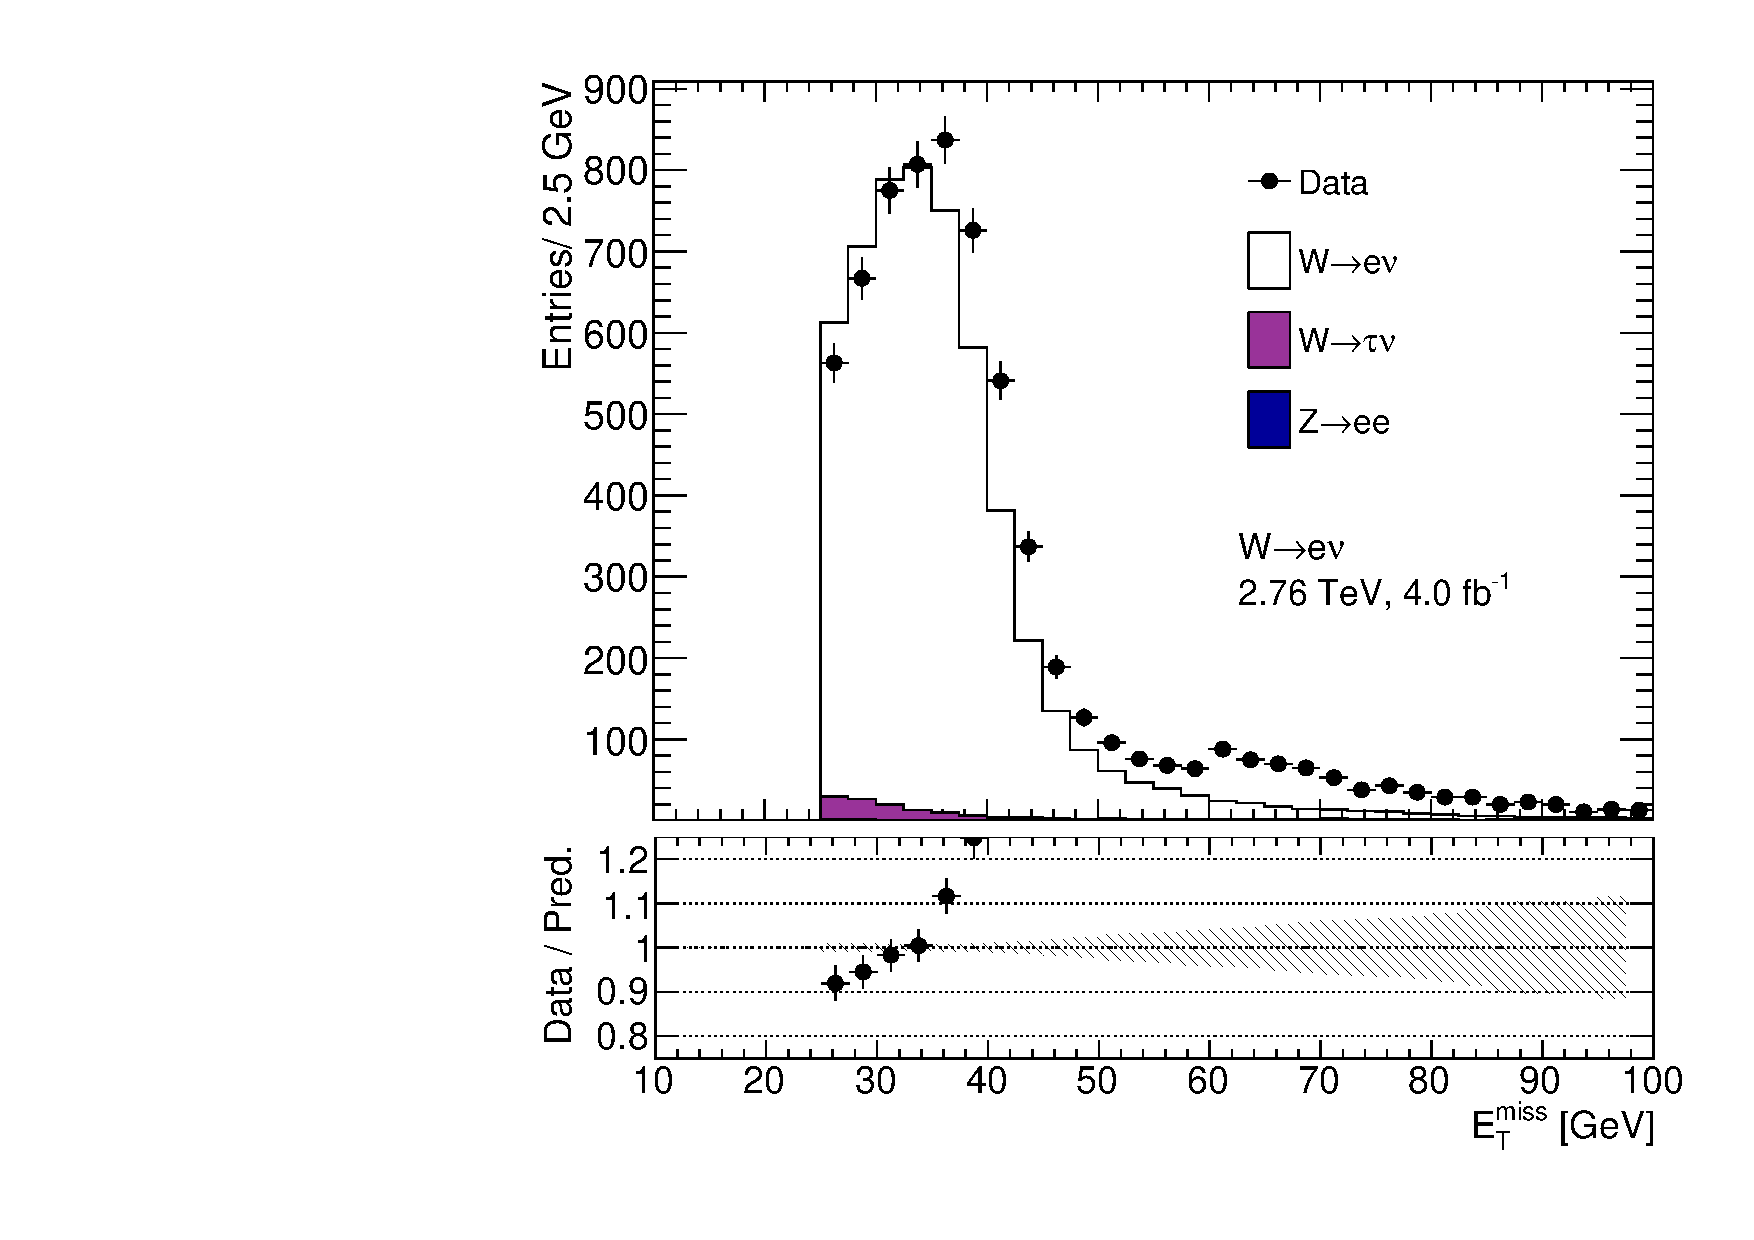
\includegraphics[width=1.\linewidth]{HadronRecoil/WenuRefFinal.pdf} \\ a)}
\end{minipage}
\hfill
\begin{minipage}[h]{0.49\linewidth}
\center{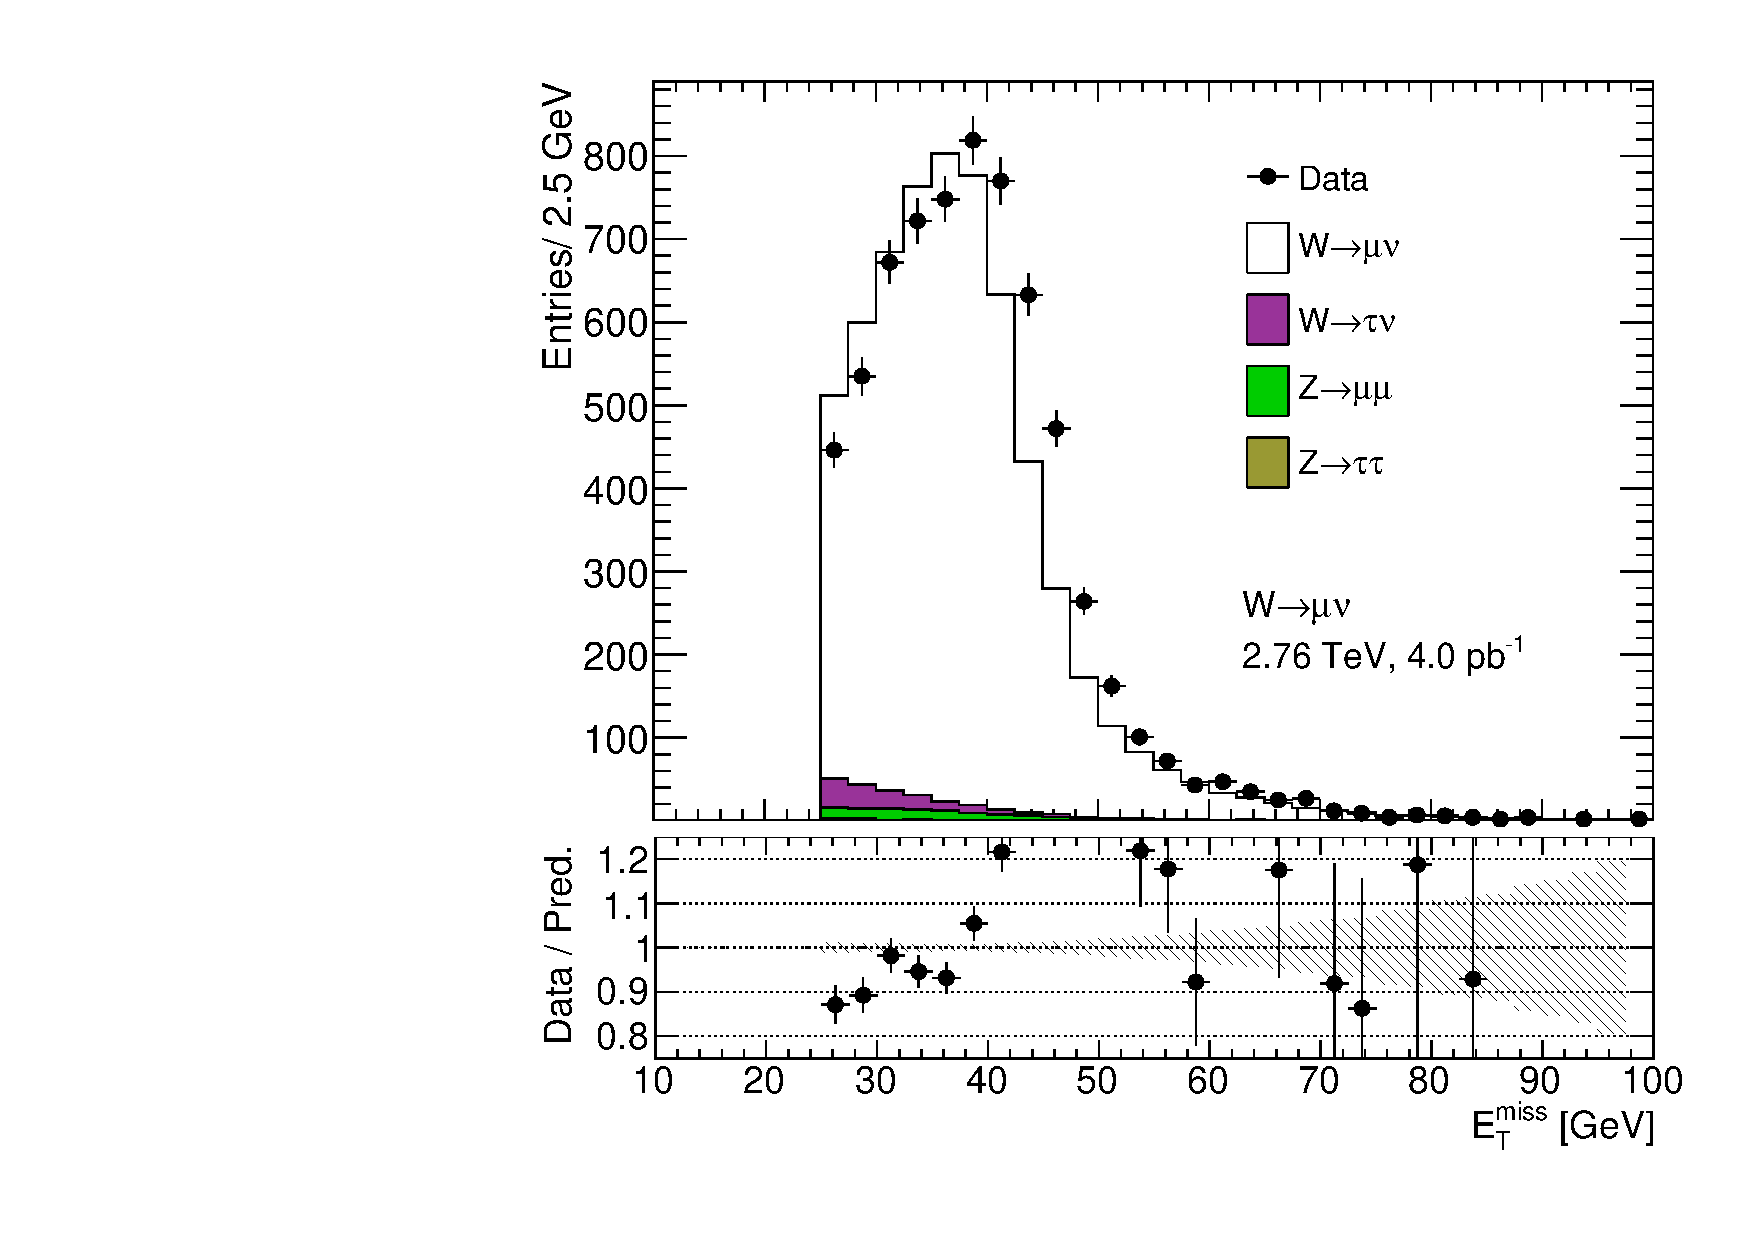
\includegraphics[width=1.\linewidth]{HadronRecoil/WmunuRefFinal.pdf} \\ b)}
\end{minipage}
\caption{Data and MC comparison for \etmiss calculated by standard \atlas algorithm for a)\wenu b)\wmunu events}
\label{ris:EtMissRefFinal}
\end{figure}
This procedure was optimised for 8 TeV runs  and using a calibration constants from it. This can cause problems with 2.76 TeV low pileup run. As a examine showed this is not optimal procedure in this case. Control plots for W production in electron and muon channels are shown on a  Fig. \ref{ris:EtMissRefFinal}. Where a big discrepancies in a muon and electron channel, that cannot be accounted to multijet background. 

\begin{figure}[t]
\begin{center}
\begin{minipage}[h]{0.49\linewidth}
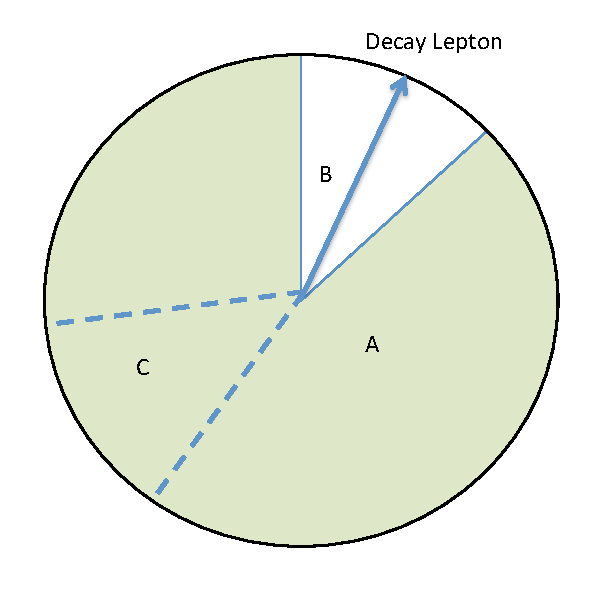
\includegraphics[width=1\textwidth]{HadronRecoil/ReplacementCluster.pdf}
\end{minipage}
\hfill
\begin{minipage}[h]{0.49\linewidth}
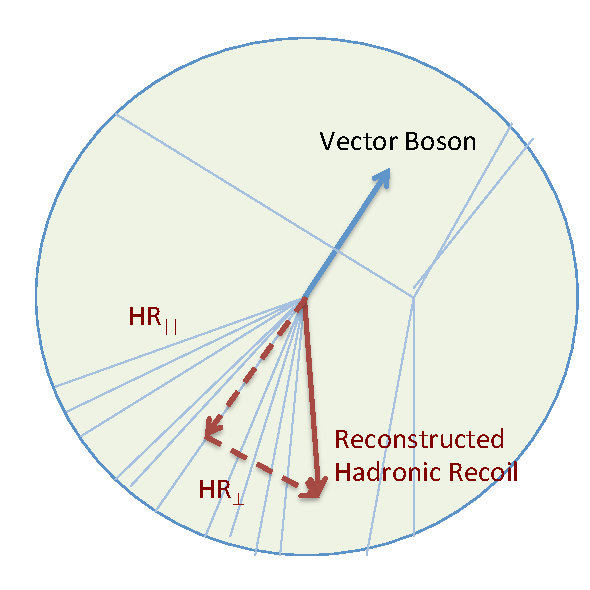
\includegraphics[width=1\textwidth]{HadronRecoil/RecoHRParPerp.pdf}}
\end{minipage}
\caption{a) Definition of different zones in the calculation of the cluster-based hadronic recoil. \label{ris:subsCone}, b) Parallel and perpendicular projection of the hadronic recoil with the respect to the transverse momentum of the vector boson \label{ris:HadrRecoilTruthPt}}
\end{center}
\end{figure}


\section{Hadron Recoil Calculation}
Second way of calculating \etmiss was developed specifically for a W and Z decays by W mass measurements group. This procedure is using this fact, that a transverse momentum of a W-boson has to be balanced with initial (quark-gluon) state radiation, because initial sum of transverse momentum is zero:
\begin{equation}
\vec{P_{T}^{W}} = \vec{P_T^{lep}}+\vec{P_T^{\nu}}= \sum{\vec{P_{T}^{ISRquarks,gluon}}}, 
\end{equation}
where $\sum{\vec{P_{T}^{ISRquarks,gluon}}}$ is a transverse momentum of partons from initial state radiation, also called hadronic recoil (HR). Therefore, \etmiss can be determined as:
\begin{equation}
E_{T}^{miss} = P_T^{\nu} =  - HR + p_T^{l}
\end{equation} 

This procedure assumes, that recoil is arises from one single leading jet, and the rest  is coming from a soft hadronic activity. This hadron recoil is computed as a vector sum of calorimeter clusters:
\begin{equation}
HR= \sum_{i=0}^{N_{topo}}\vec{p_T^{topo}}
\end{equation}
while a scalar sum of all transverse energies is corresponding to the hadronic activity of the event:
\begin{equation}\label{eq:sumet}
\sum E_T =\sum_{i=0}^{N_{topo}} E_T^{topo}
\end{equation}
To avoid double counting of lepton energy losses in calorimeter, the clusters inside cone with radius dR = 0.2 are excluded from this calculation.To compensate soft activity inside this cone, clusters are then compensated by replacement cone (Fig. \ref{ris:subsCone}). This cone is defined as cone at the same pesudorapidity, but different $\phi$. It should be far from any other lepton and hadron recoil direction. Each cone is then rotated to a direction of the original lepton direction. This definition is not taking into account jet reconstruction aspects.   This is allowing to get a better data MC agreement (Fig. \ref{ris:HadrRecoilEtMiss}).


\begin{figure}[b]
\begin{minipage}[h]{0.49\linewidth}
\center{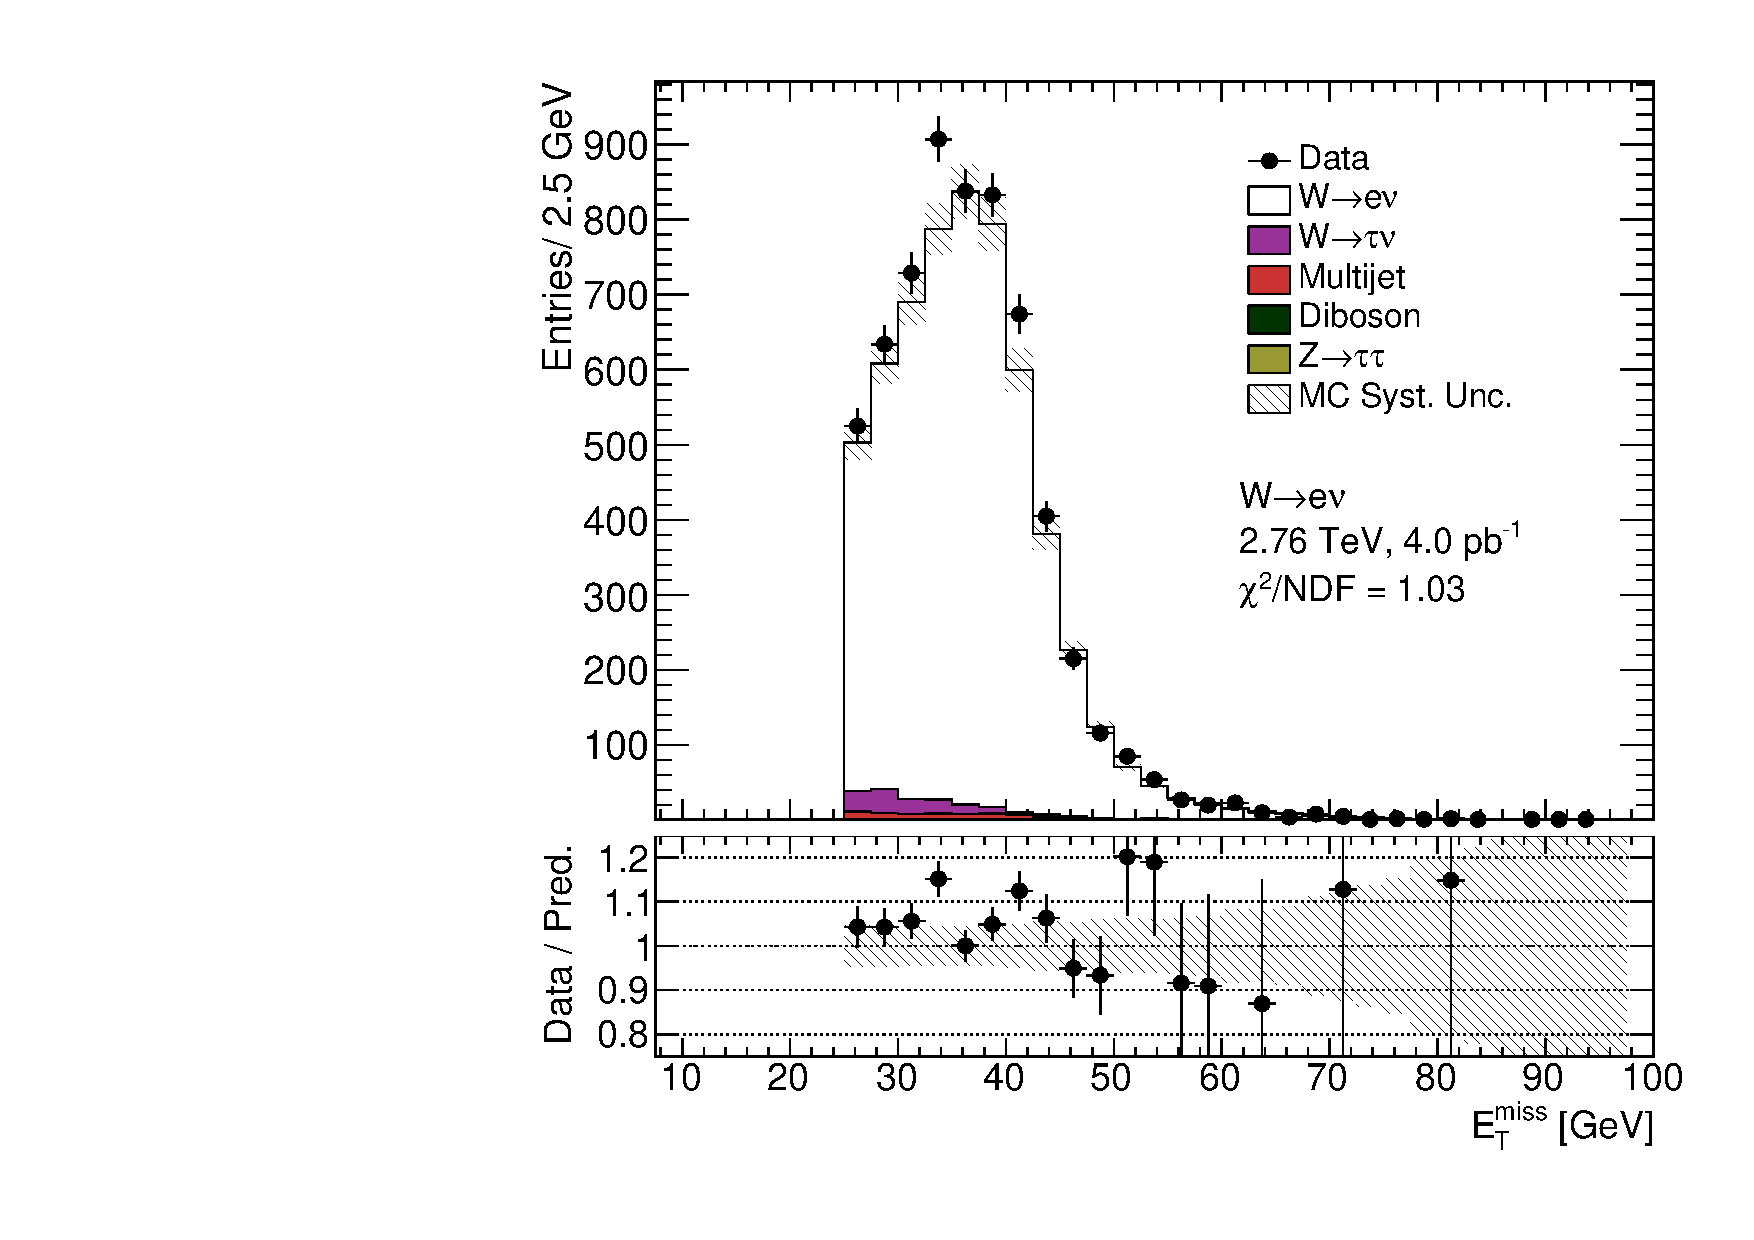
\includegraphics[width=1.\linewidth]{HadronRecoil/W_Boson_etMiss.pdf} \\ a)}
\end{minipage}
\hfill
\begin{minipage}[h]{0.49\linewidth}
\center{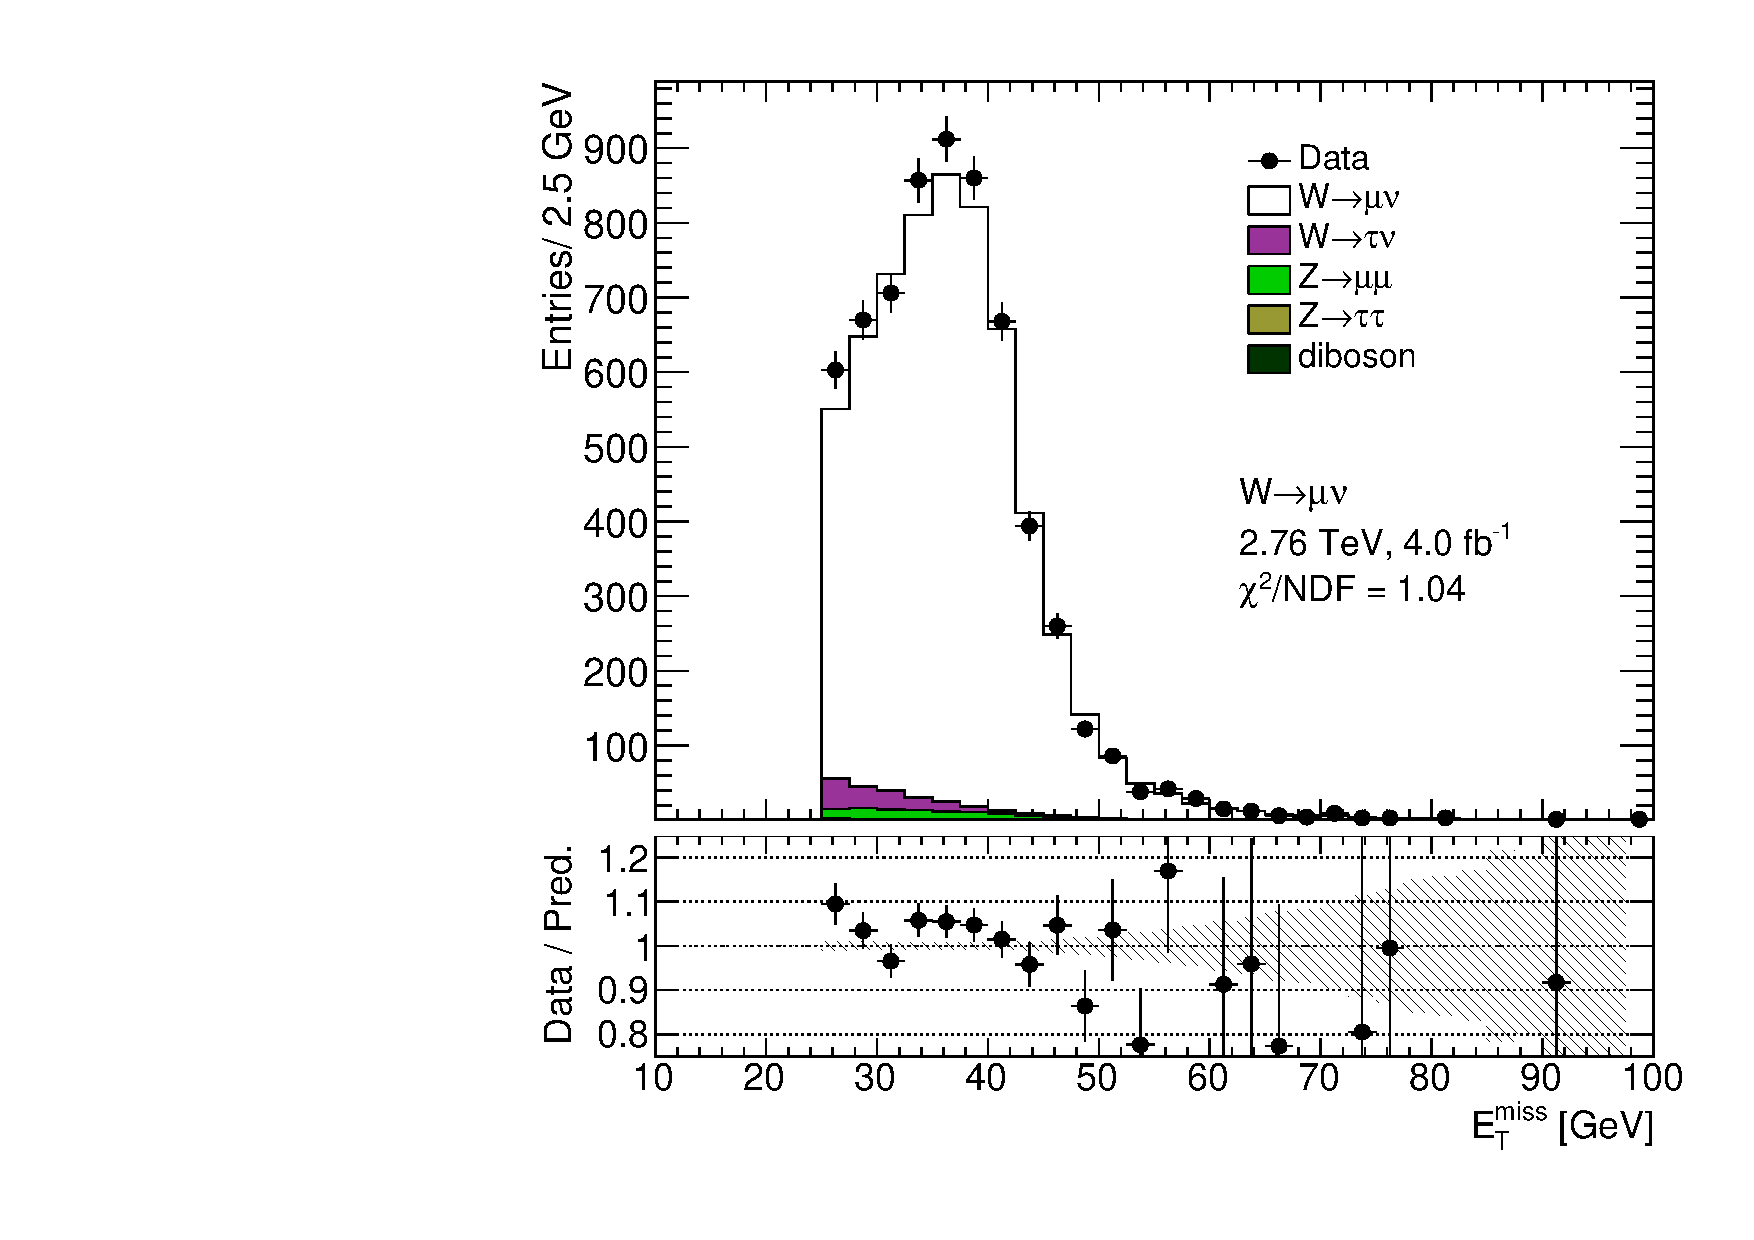
\includegraphics[width=1.\linewidth]{HadronRecoil/Wmu_Boson_etMiss.pdf} \\ b)}
\end{minipage}
\caption{Data and MC comparison for \etmiss calculated from hadron recoil for a)\wenu b)\wmunu events}
\label{ris:EtMissRefFinal}
\end{figure}



\section{Hadron Recoil calibration}
\etmiss affects significantly on a W boson measurement, so its important to have good understanding of sources of a possible differences in a hadron recoil reconstruction in a data and monte carlo. 

The hadron recoil algorithm performance can be studied in MC through the projection of $\vec{HR}$ on the direction of the transverce momentum of the vector boson, as shown on Fig. \ref{ris:HadrRecoilTruthPt}. This projection can be divided into perpendicular \uperp and a parallel \upar component as follows:
\begin{equation}
\upar=\vec{v_{xy}}\cdot\vec{HR}
\uperp=v_x\cdot HR_y - v_xy \cdot HR_x,
\end{equation}
where $\vec{v_xy}$ is a transverse component of vector boson direction and $v_x$ and $v_y$ are the projections on x and y plane respectivelly. In ideal case this $\upar=p_T^{bos}$ and $\uperp = 0$. However calorimeter resolution is causing relativelly wide distributions for this projections (Fig. \ref{somethig}). Parallel component \upar is sensitive to a possible bias in the hadron recoil, while perpendicular \uperp can be used for a determination of resolution discrepancies. The mean and width of this distributions can depend on a different variables, such as mean number of interactions in event, hadronic activity, boson $P_{T}^{bos}$ etc. Typical resolution of measured hadron recoil is <something>

\begin{figure}[t]
\centering
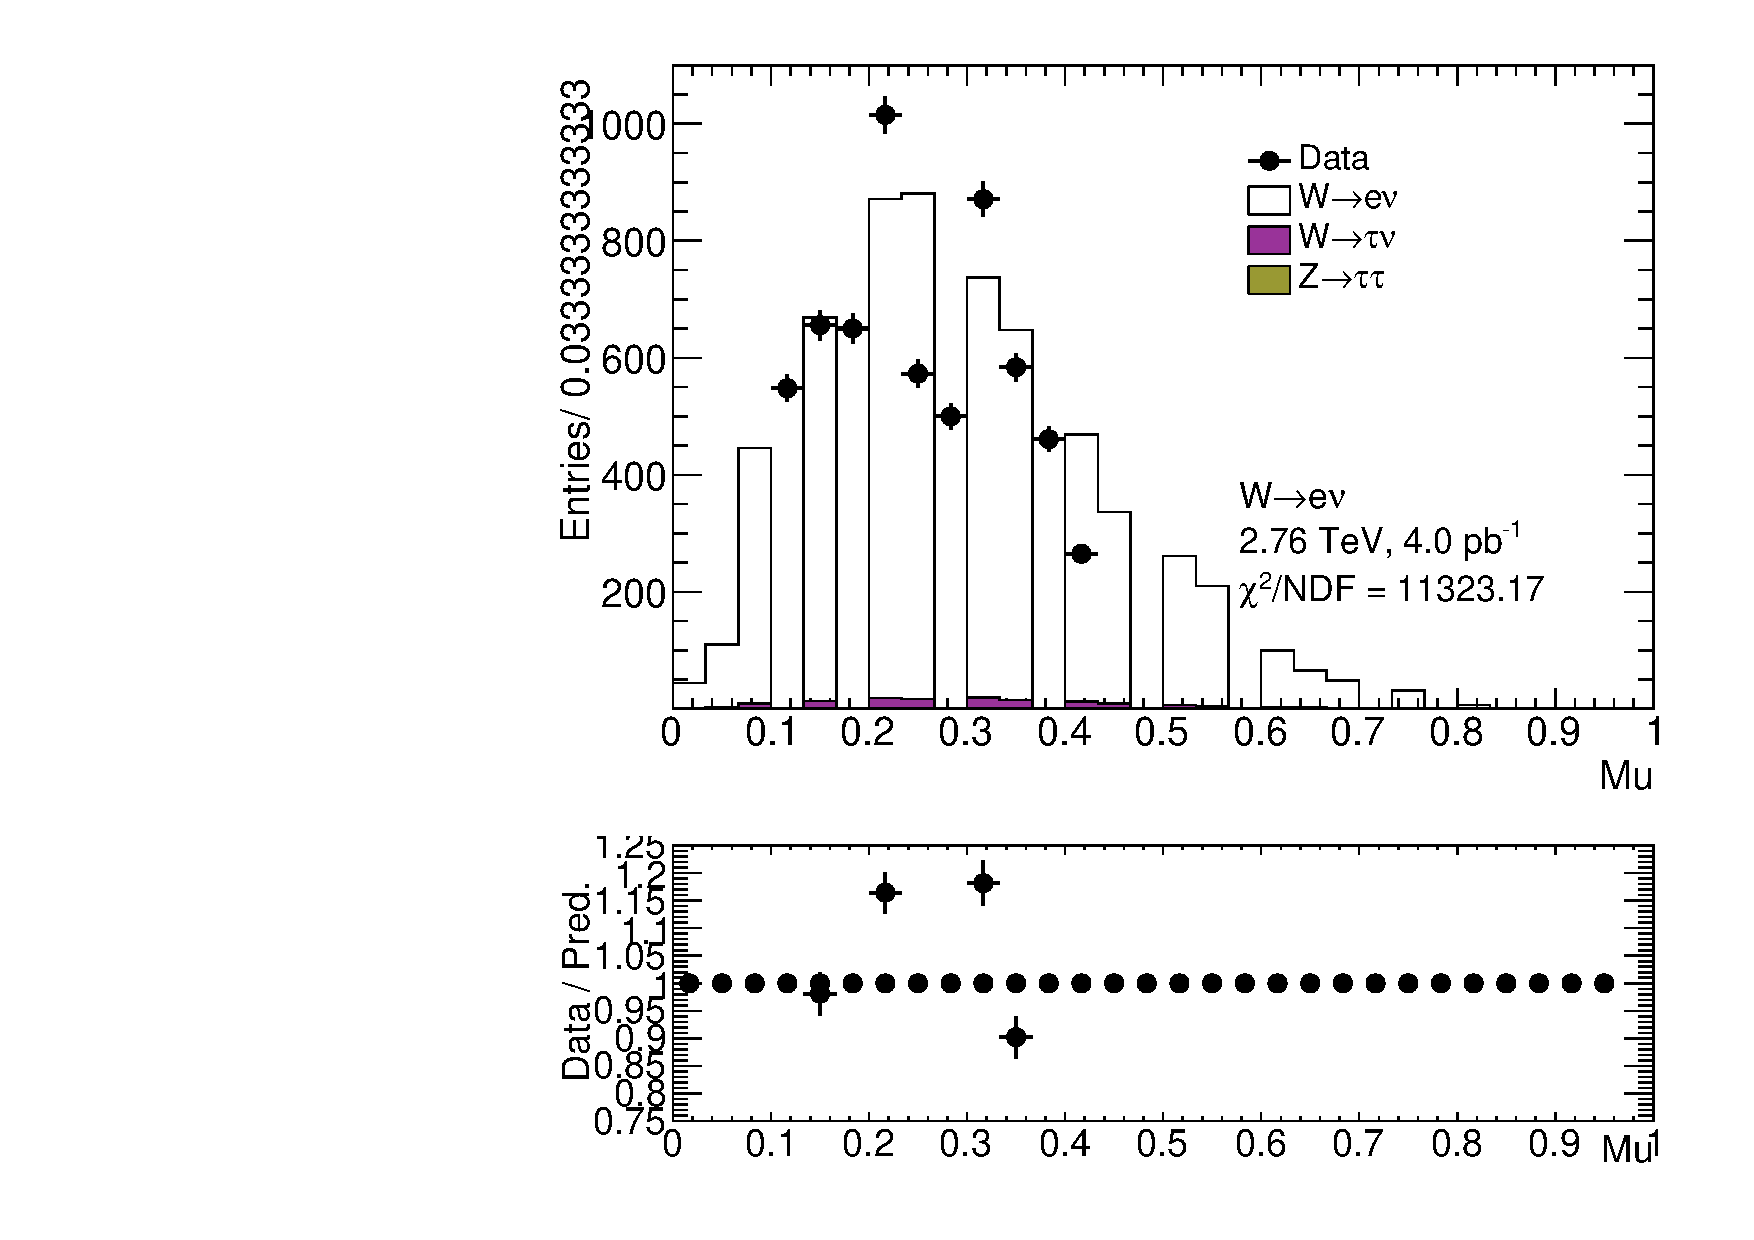
\includegraphics[width=0.5\textwidth]{HadronRecoil/W_Event_Mu.pdf}
\caption{Pileup}
\label{HadrRecoil:mu}
\end{figure} 
 
It is convinient to use Z boson decays for a hadron recoil calibration, since its transverse momentum can be determined not only by a hadron recoil, but also from its decay products.  Zpt resolution coming from lepton reconstruction is 3-4 times better, than from a hadron recoil. This is allowing to treat leptonically reconstructed $P_T^{Z}$ as a truth $P_T$ of the boson and compare directly \uperp and \upar in data and MC. Small size of the Z sample in 2.76TeV data will lead to a high statistics error for this distributions. Also, calibration constants can be also derived from W boson decays through the indirect measurments. This corrections can be biased by a possible truth boson $P_T$ mismodelling. 
 
 First step in a hadron recoil calibration procedure ames to correct differences in a pile-up modelling in the event. Additional interaction can have a significant effect on a \etmiss and \sumet distributions.   It is usually accounted scaling average number of interaction per bunch crossing to match a data. However, \atlas simulation is suited for an high pile-up runs, so this quantity is modelled discretly in case of 2.76 TeV analysis (Fig. \ref{HadrRecoil:mu}), what makes the corrections to match data impossible. 

The combined Z and W boson determination procedure have been used. This section describes a procedure of calibrating bias and resolution mismodelling in a hadron recoil, that was apapted for 2.76 TeV data. 

\subsection{Hadron recoil resolution correction}
There are two possible ways of correcting hadron recoil resolution in a 2.76 TeV data. 

Event activity plays an important role in a \etmiss reconstruction. Since \sumet and hadron recoil resolution values are correlated, the possible mismodelling of event activity can lead to a differences between data and monte carlo (Fig. \ref{sumet}). It could be corrected by reweigting \sumet distribution to match a data (blue arrow on a Fig.). Remaining differences can be corrected on a second step. On another hand it is also possible to neglect second order effects on \etmiss from \sumet distribution and directly correct difference between data and MC (red arrow on a Fig).

\subsubsection{Sumet distribution correction}

Distribution of \sumet  events are shown on a Fig. \ref{HadrRecoil:UncorrSumet}. There is a clear sign of shift in this distribution in a both channels. Unfortunatelly, size of the Z sample is not sufficient for correcting this discrepancies. 
The determination of sumet reweighting constants uses W boson decays. This procedure should leave the truth boson Pt spectrum untouched. In order to do so, the correction factor are derived inside pt bins as follows:
\begin{equation}
SF^{channel}=\frac{\sum E_T^{data,\, selection} }{\sum E_T^{MC,\, no\, cuts} },
\end{equation}
where $\sum E_T^{data,\, selection} $ and $\sum E_T^{MC,\, no\, cuts}$ is a \sumet distribution inside $p_T^{W, rec}$ bin without any cuts. Oppositely, in MC $\sum E_T^{MC,\, no\, cuts} $ is taken without any cuts. Scale factors are determined separatelly for each signal process for a W boson decays.  In order to increase statistics in data the combination of \wenu and \wmunu processes is used.  In order to have a smother correction and not try to account data fluctuation ratio inside each bin can be parameterised by a polynomial degree   2 inside each $p_T^{W, rec}$ bin (Fig. \ref{something}).  Total SF obtained by this procedure are shown on a Fig. \ref{something}. The distribution of \sumet after correction is shown on a Fig. \ref{HadrRecoil:CorrSumet}. Reconstructed boson pt spectrum is leaving almost untouched, while this procedure still intoduses some shift in a truth boson pt spectrum(Fig. \ref{HadrRecoil:PtSpectrum} ). Effect on the resoultion of \uperp is shown on a Fig. \ref{something}.

\begin{figure}[h]
\begin{minipage}[h]{0.40\linewidth}
\center{\includegraphics[width=1.\linewidth]{HadronRecoil/UncorrSumet/W_EtMiss_CorRecoilSumet.pdf} \\ a)}
\end{minipage}
\hfill
\begin{minipage}[h]{0.40\linewidth}
\center{\includegraphics[width=1.\linewidth]{HadronRecoil/UncorrSumet/Wmu_EtMiss_CorRecoilSumet.pdf} \\ b)}
\end{minipage}
\label{HadrRecoil:UncorrSumet}
\vfill
\begin{minipage}[h]{0.40\linewidth}
\center{\includegraphics[width=1.\linewidth]{HadronRecoil/CorrSumet/W_EtMiss_CorRecoilSumet.pdf} \\ a)}
\end{minipage}
\hfill
\begin{minipage}[h]{0.40\linewidth}
\center{\includegraphics[width=1.\linewidth]{HadronRecoil/CorrSumet/Wmu_EtMiss_CorRecoilSumet.pdf} \\ b)}
\end{minipage}
\caption{}
\label{HadrRecoil:CorrSumet}
\end{figure}


\begin{figure}[t]
\centering
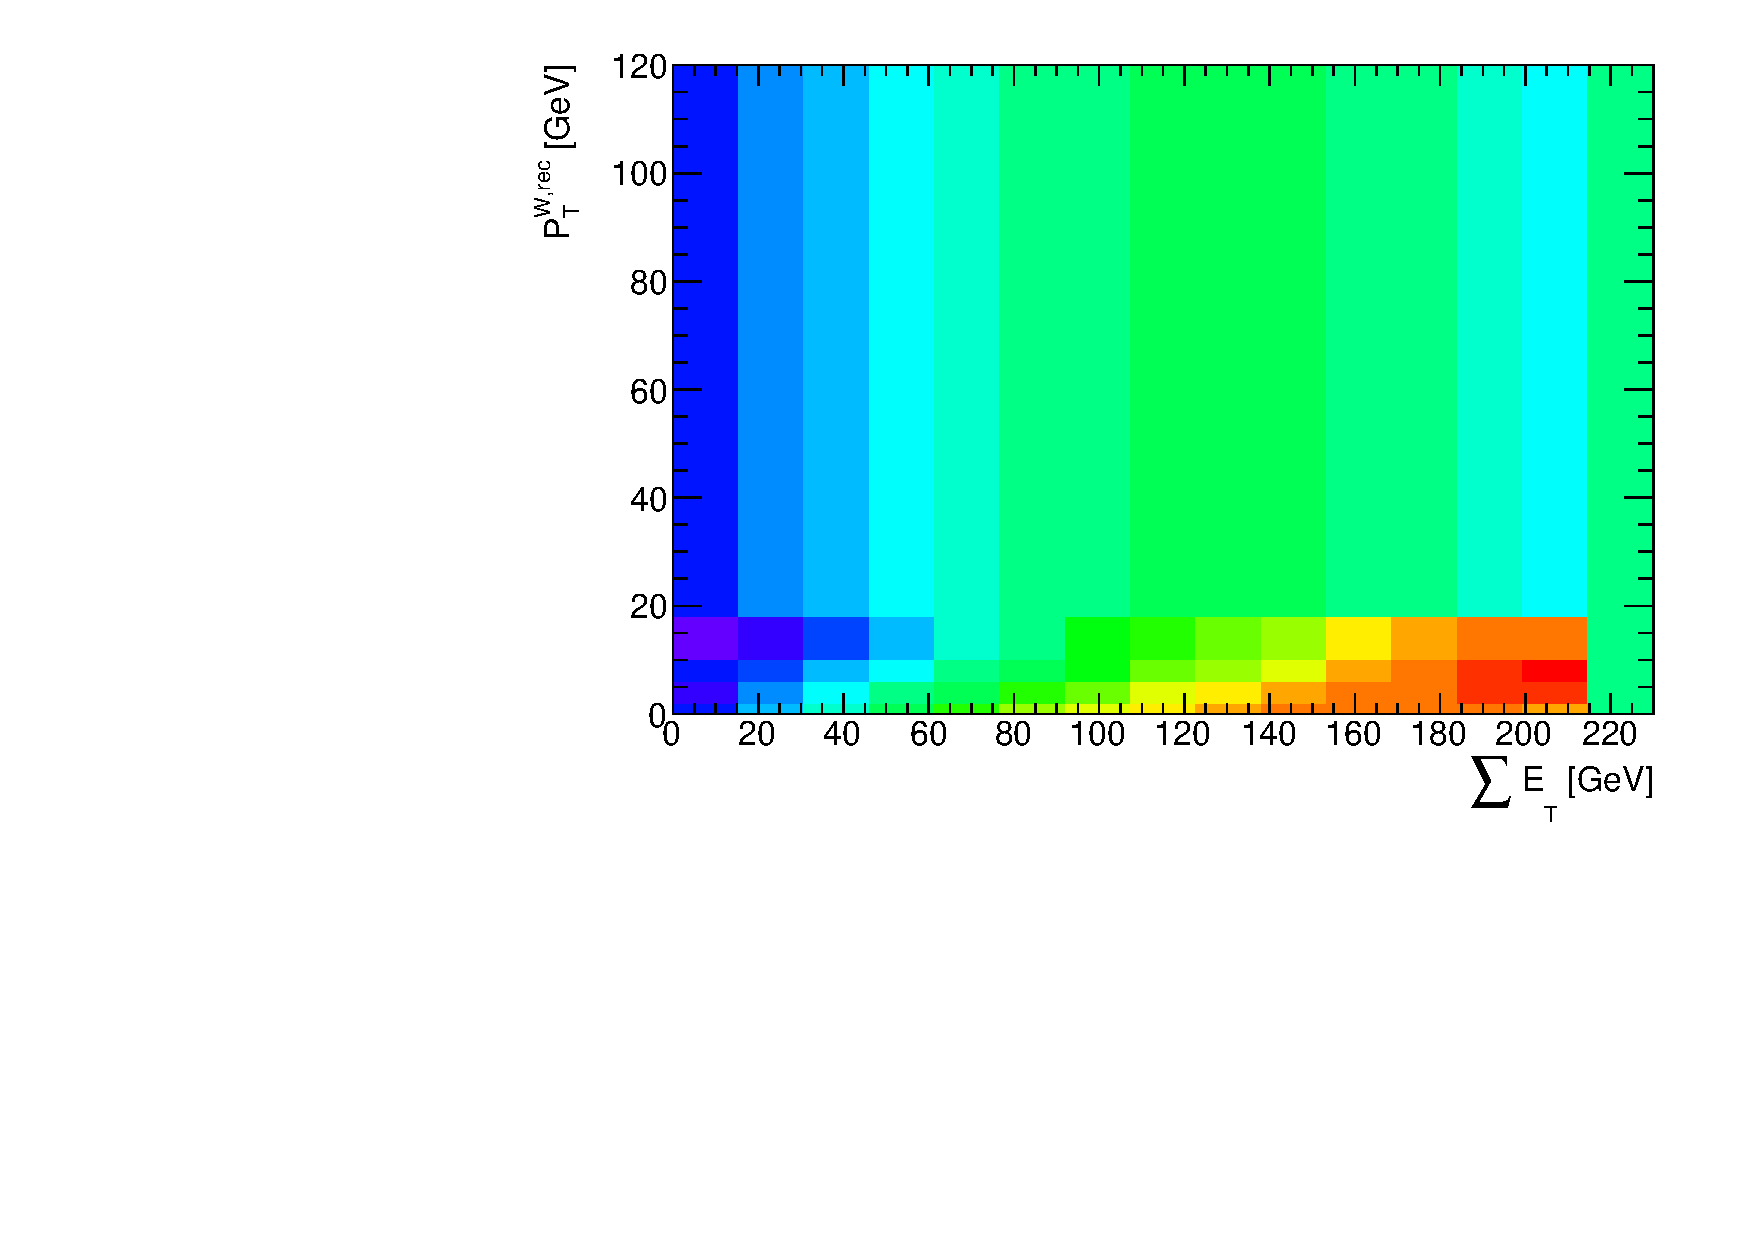
\includegraphics[width=0.7\textwidth]{HadronRecoil/SF_EP.pdf}
\caption{Correction factors for \wenu}
\label{SFWplusenu}
\end{figure}

Statistical error of this fluctuations can be estimated from polynomial parameters obtained from fit using bootstrap method. Inside each bin parameters are varied within its fit uncertanty as:
\begin{equation}
fit parameters new = fit parameters + gaus^{2D}(cov.matrix),
\end{equation}
where $fit parameters$  is a vector of best fit parameters and $gaus^{3D}$ is a 3D gaus, that takes covariance matrix from fit results. This method is allowing to take into account correlations between parameters. This procedure is repeated 25 times for each bin, that gives us set of 25 scale factors, that are later used for error determination.

Sytematical error can be studied by applying lower order of approximation on a SF or not applying it at all. The overall effect on a \cw for a different methods is shown in a Tab. \ref{SumetCW}. Results are dominated by a systematics error. Hoever, there is a difference in a sign of the effect for a different flavours of the analysis. This cannot be explained from a physical point of view, so it was decided not to use this corrections in a final analysis.
 
\begin{figure}[h]
\begin{minipage}[h]{0.49\linewidth}
\center{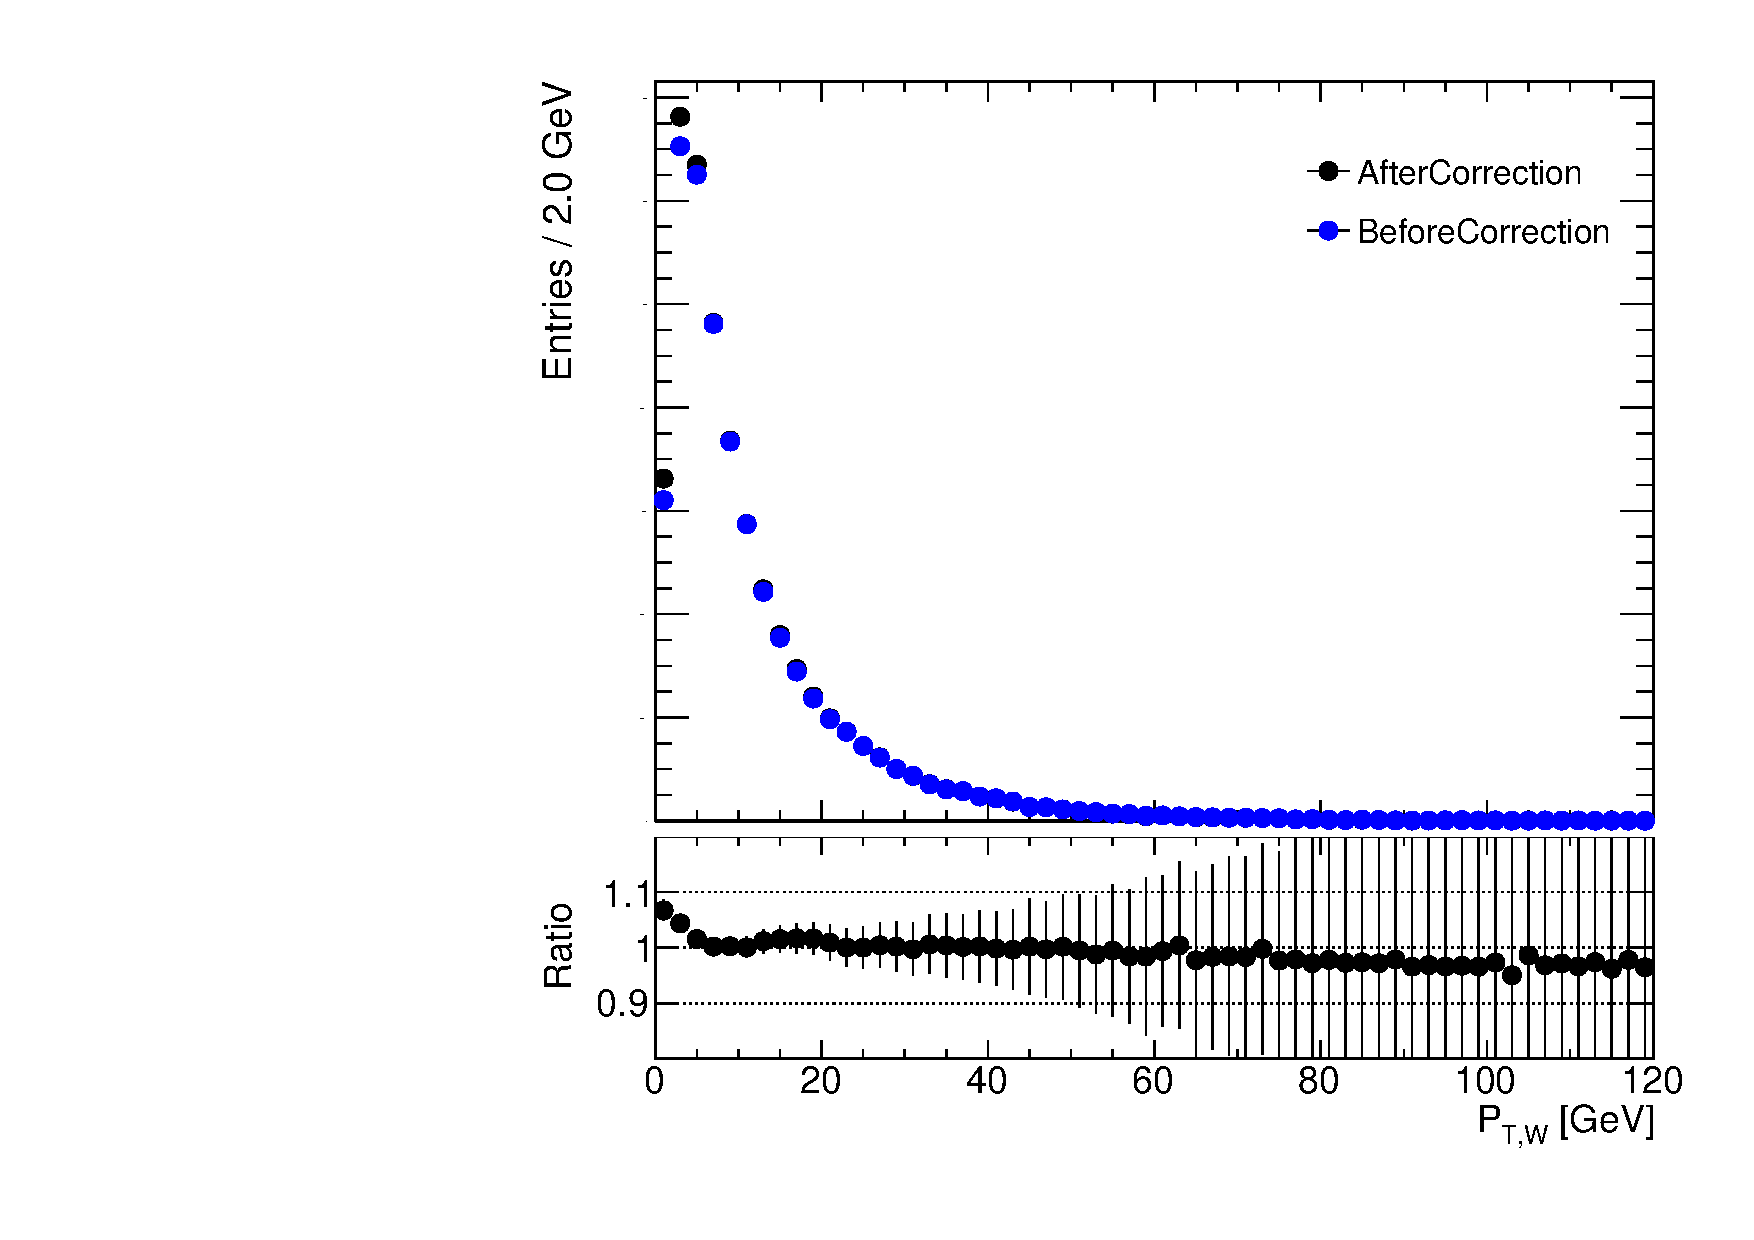
\includegraphics[width=1.\linewidth]{HadronRecoil/Wplusenu.pdf} \\ a)}
\end{minipage}
\hfill
\begin{minipage}[h]{0.49\linewidth}
\center{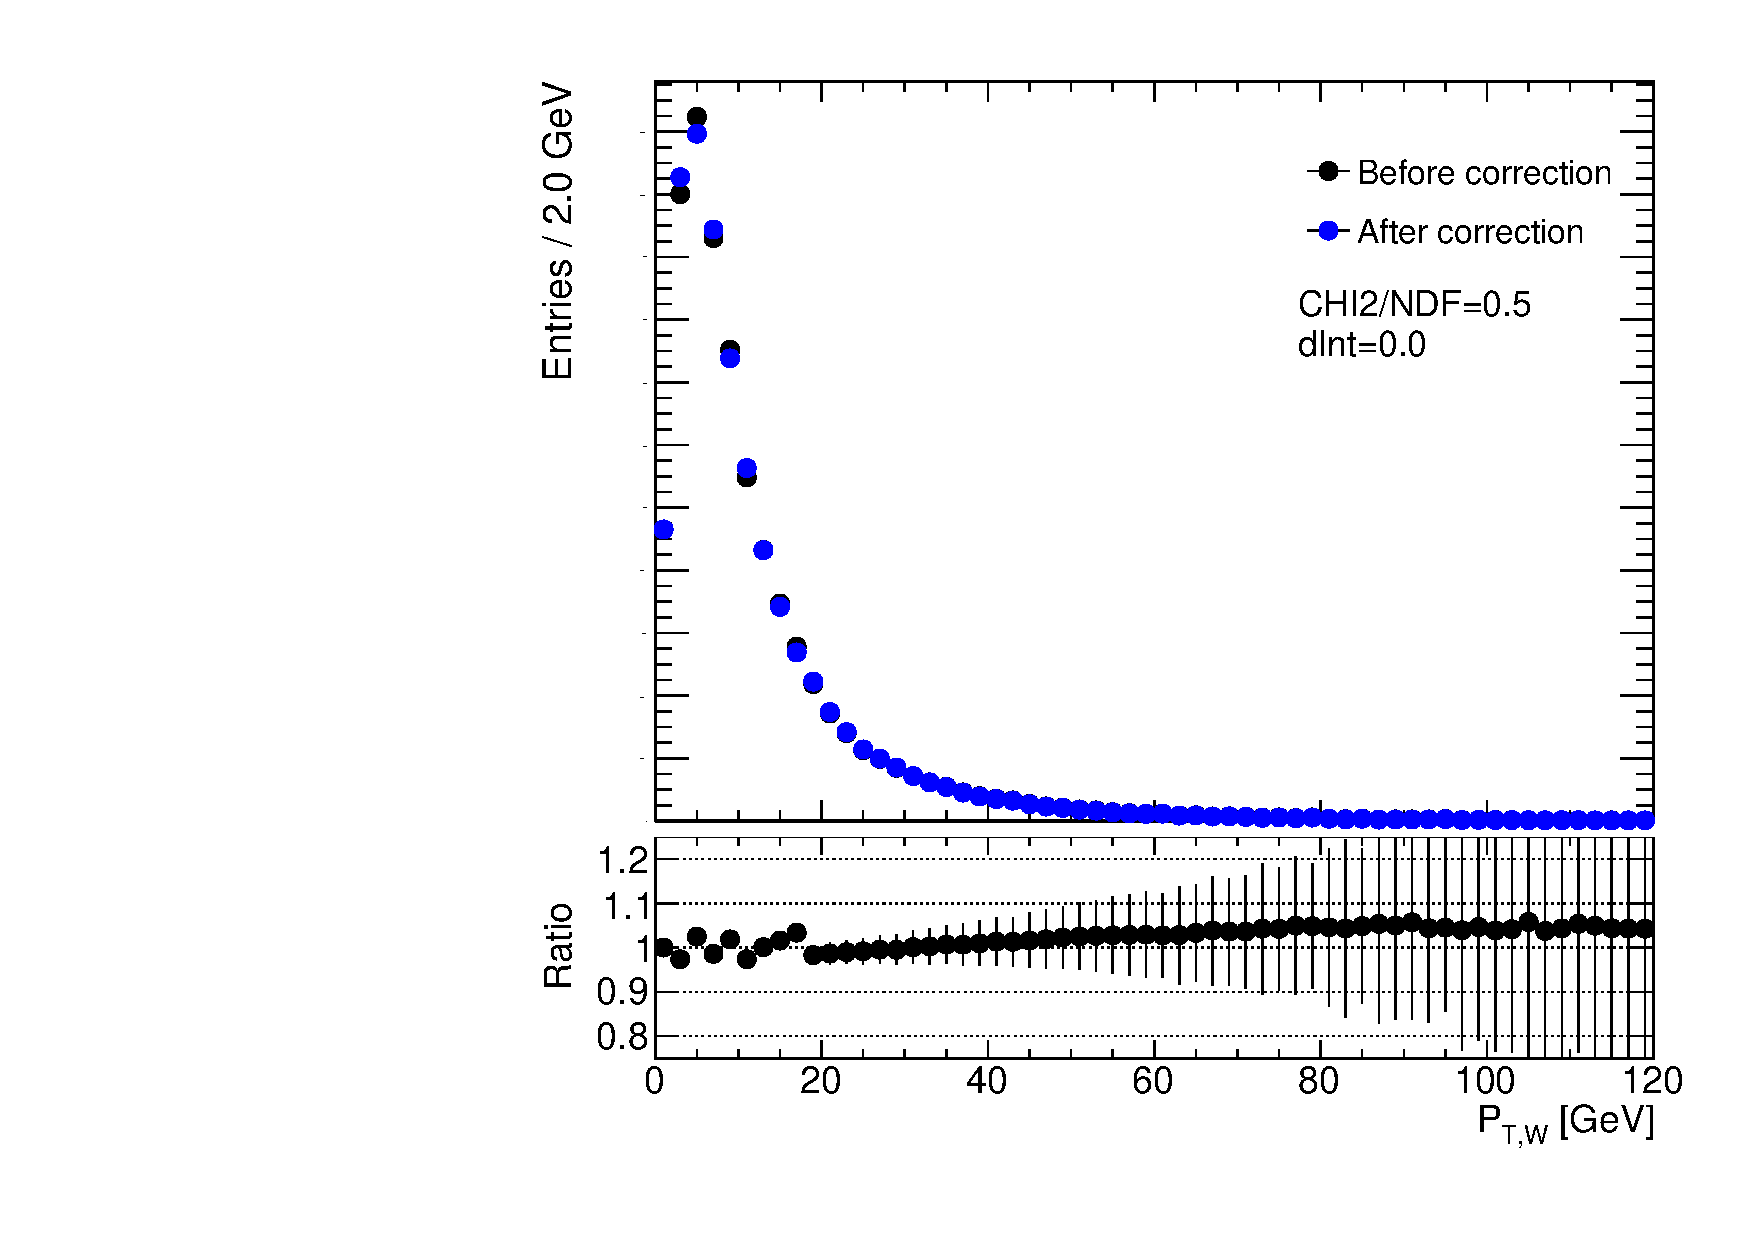
\includegraphics[width=1.\linewidth]{HadronRecoil/WplusenuRecoEffect.pdf} \\ b)}
\end{minipage}
\caption{}
\label{HadrRecoil:PtSpectrum}
\end{figure}

\subsubsection{Resolution correction using Z events}
Another way to check resolution effects is to use \uperp and \upar-$\p_T^{Z}$ distributions in a Z events. This correction assumes, that any resolution mismodelling reflects discrepancies in the \sumet distribution, while mismodelling of resolution at a given \sumet is a subleading. There is a clear difference in a rms of this distributions between data and MC, that cannot be accounted as a statistical error in data. Difference in resolutions is consistent for \uperp and $\upar- \p_T^{Z}$ distributions, but depends on a flavour of the analysis.  The resoultion mismodelling is corrected by adding up a gaus to each component of a hadron recoil:

\begin{figure}[h]
\begin{minipage}[h]{0.40\linewidth}
\center{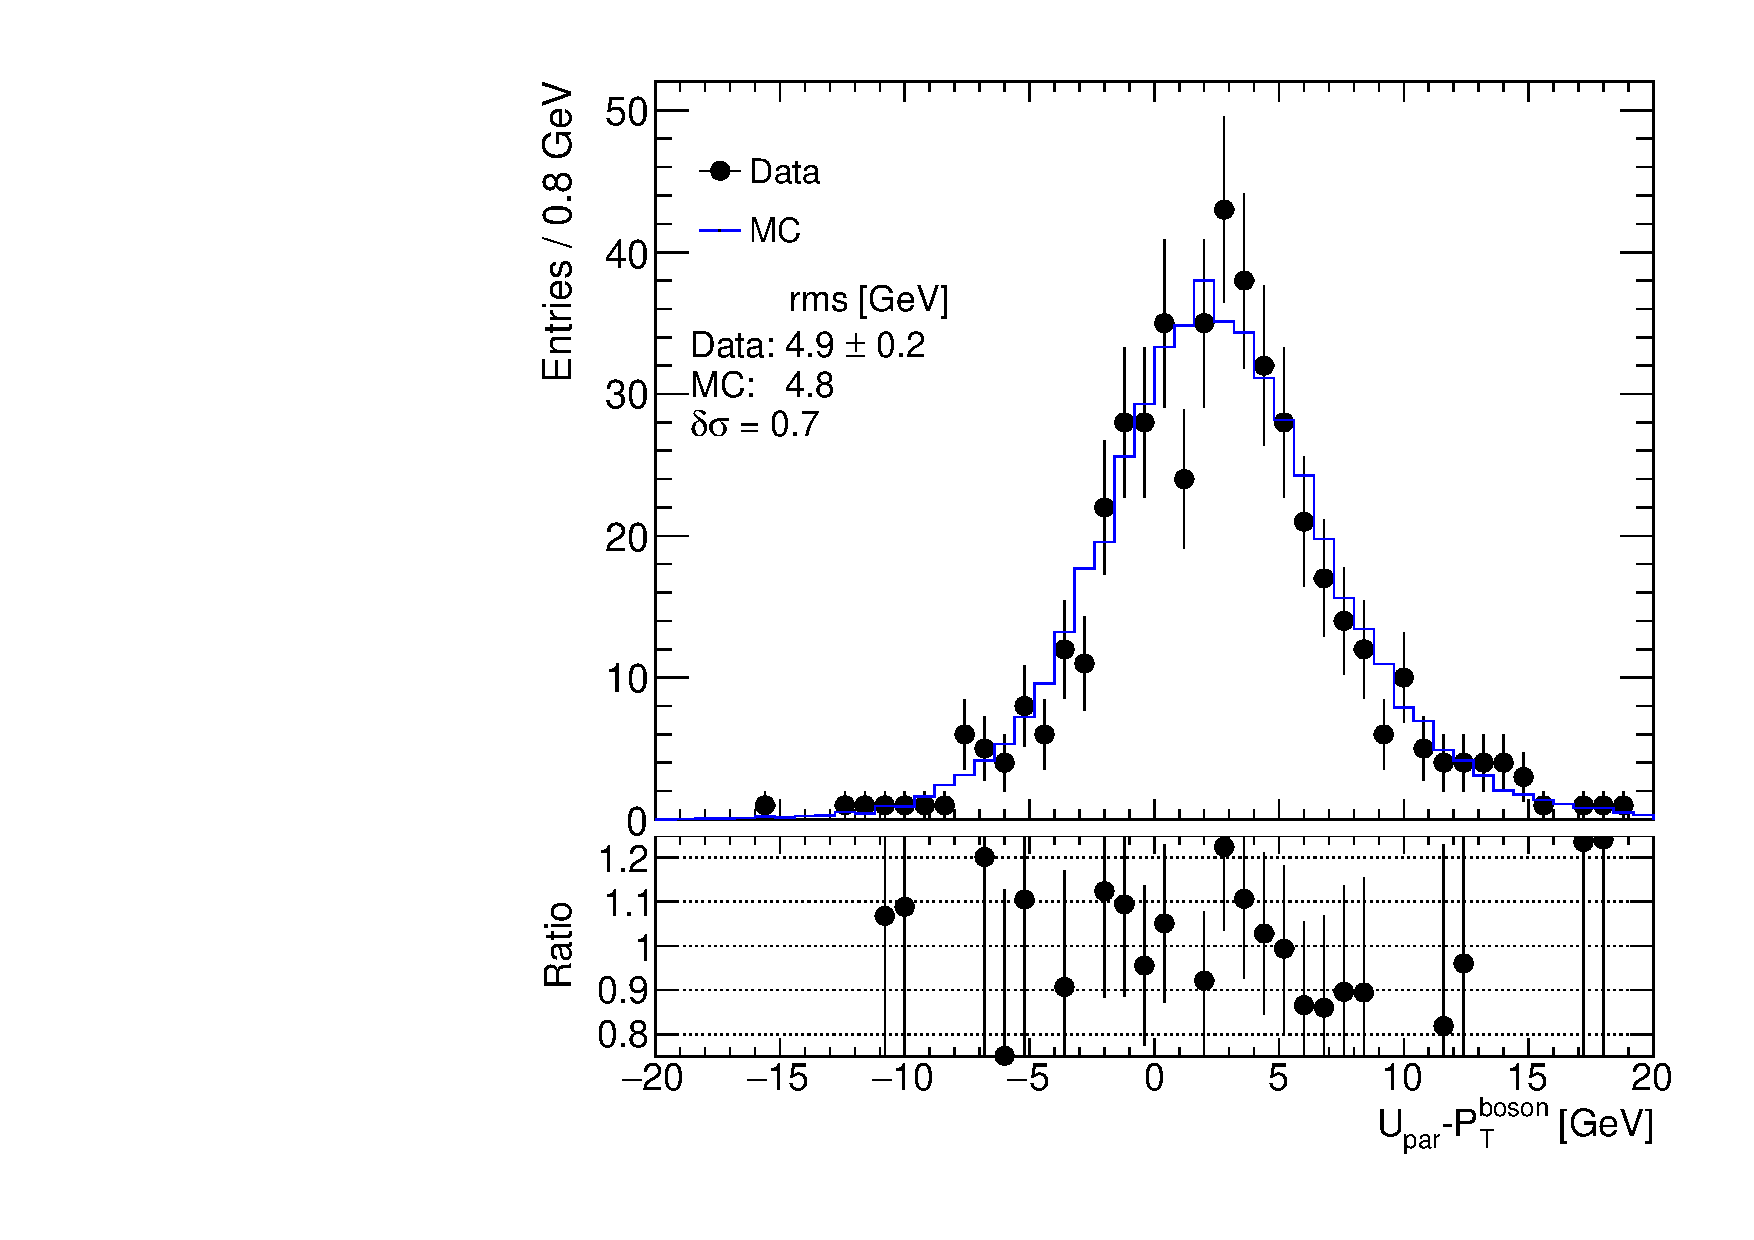
\includegraphics[width=1.\linewidth]{HadronRecoil/UParERMS.pdf} \\ a)}
\end{minipage}
\hfill
\begin{minipage}[h]{0.40\linewidth}
\center{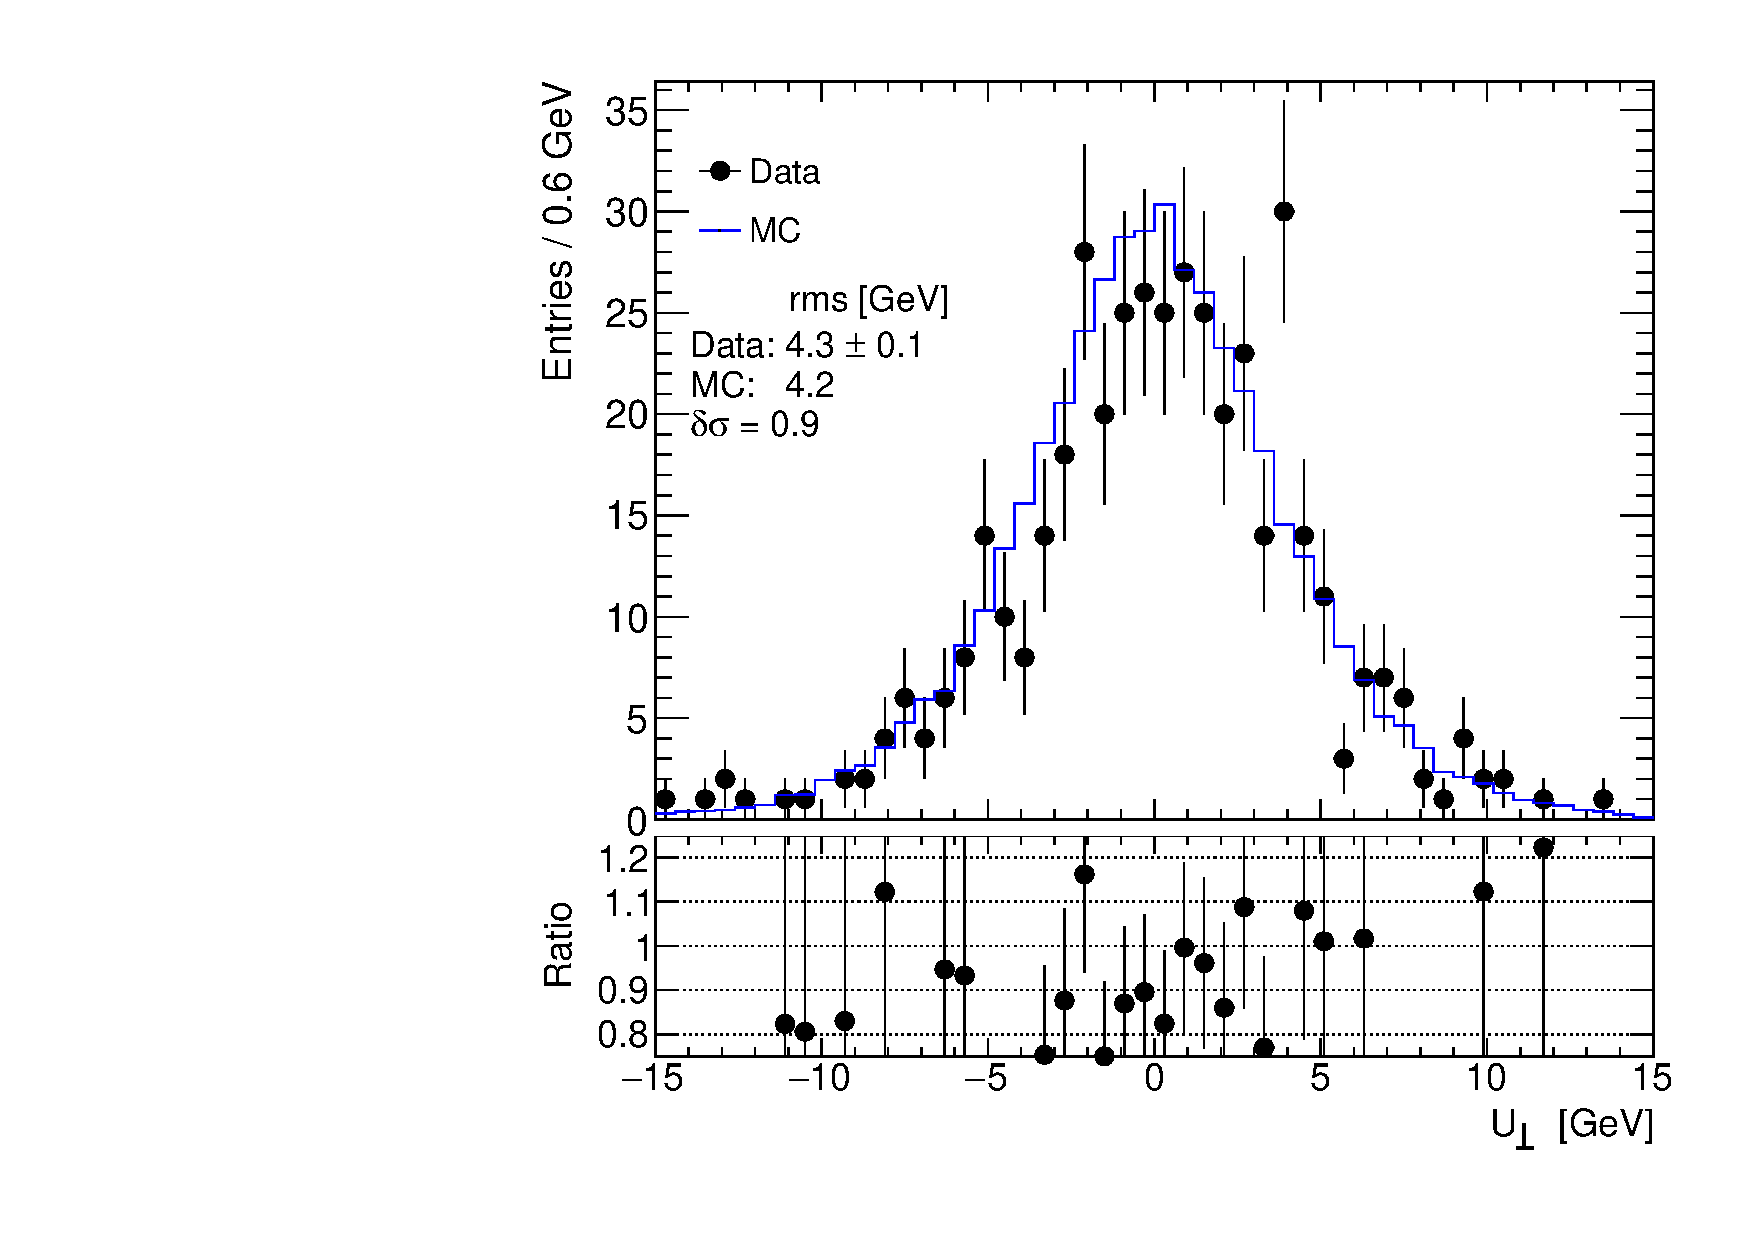
\includegraphics[width=1.\linewidth]{HadronRecoil/UPerpERMS.pdf} \\ b)}
\end{minipage}
\vfill
\begin{minipage}[h]{0.40\linewidth}
\center{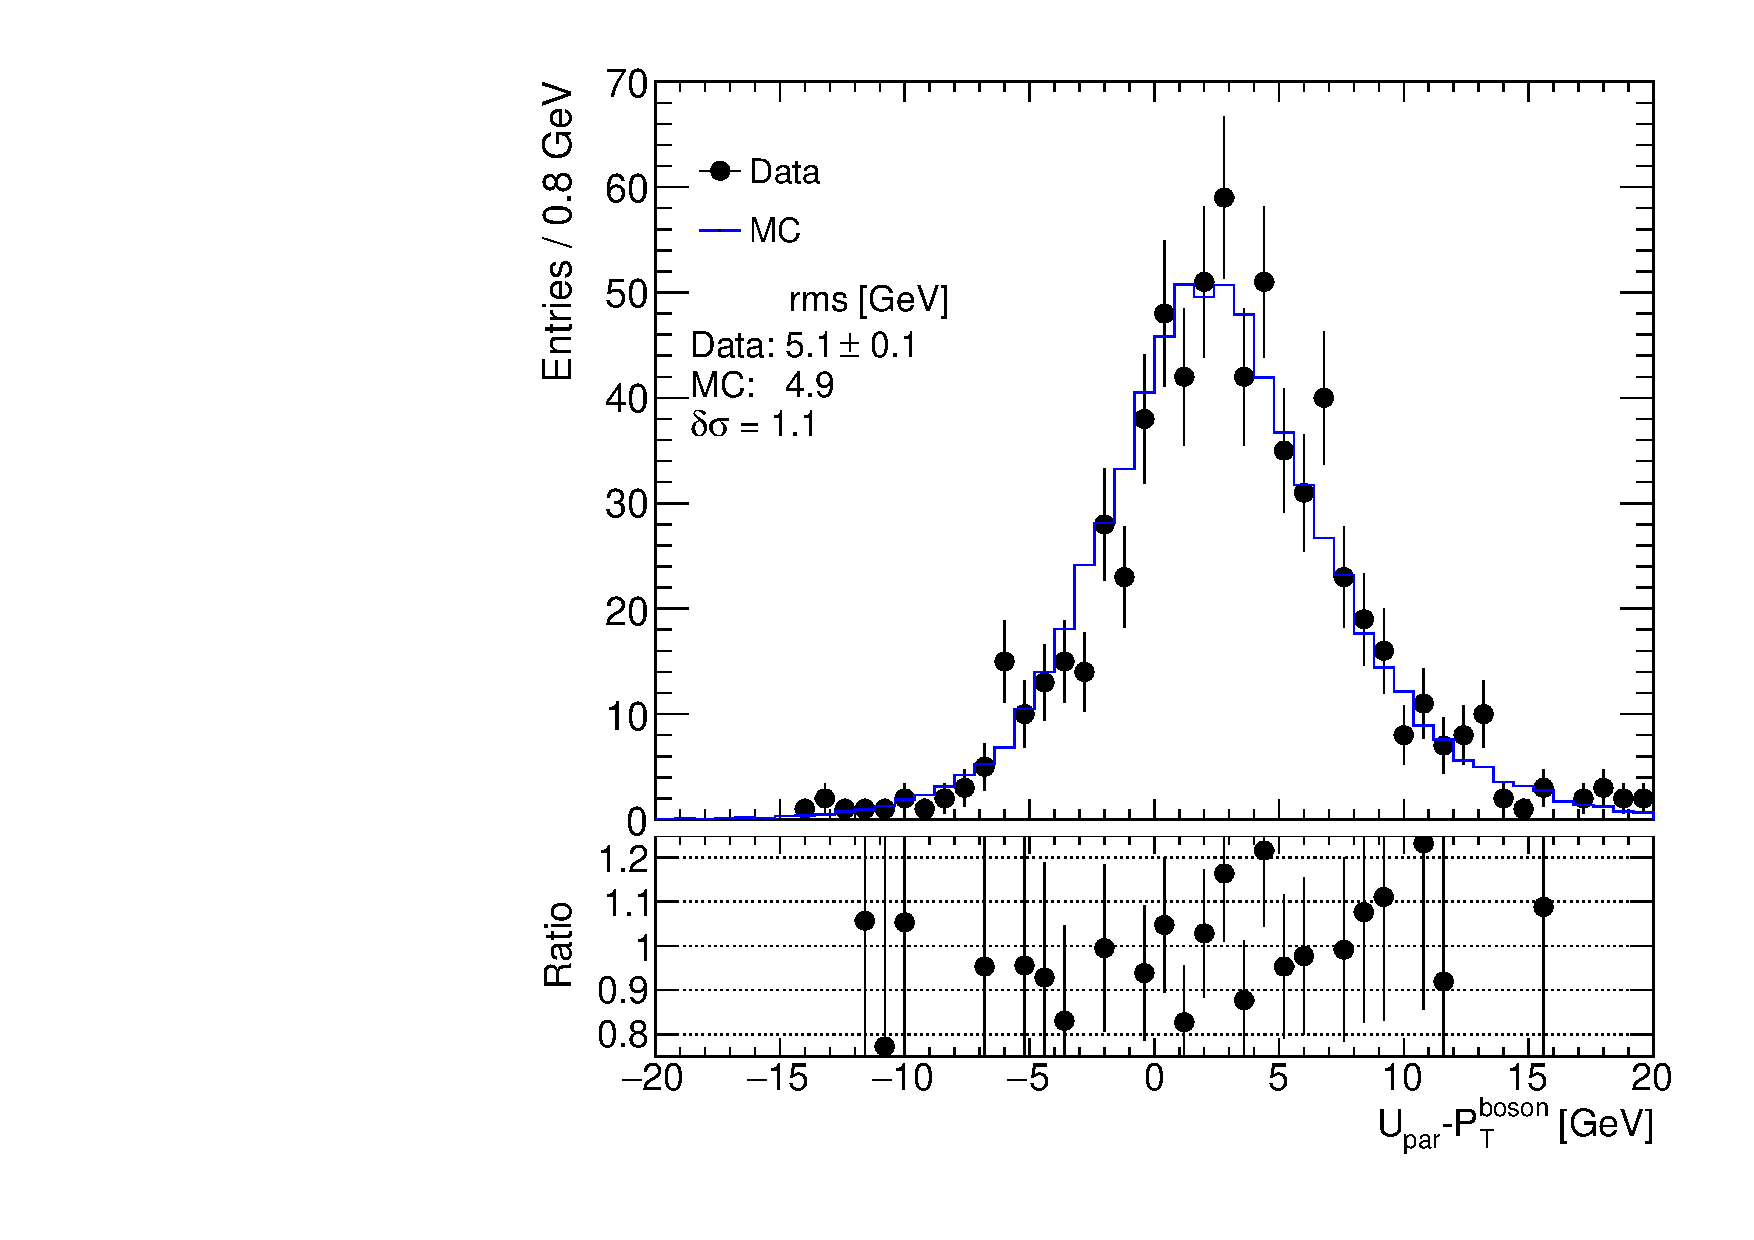
\includegraphics[width=1.\linewidth]{HadronRecoil/UParMRMS.pdf} \\ a)}
\end{minipage}
\hfill
\begin{minipage}[h]{0.40\linewidth}
\center{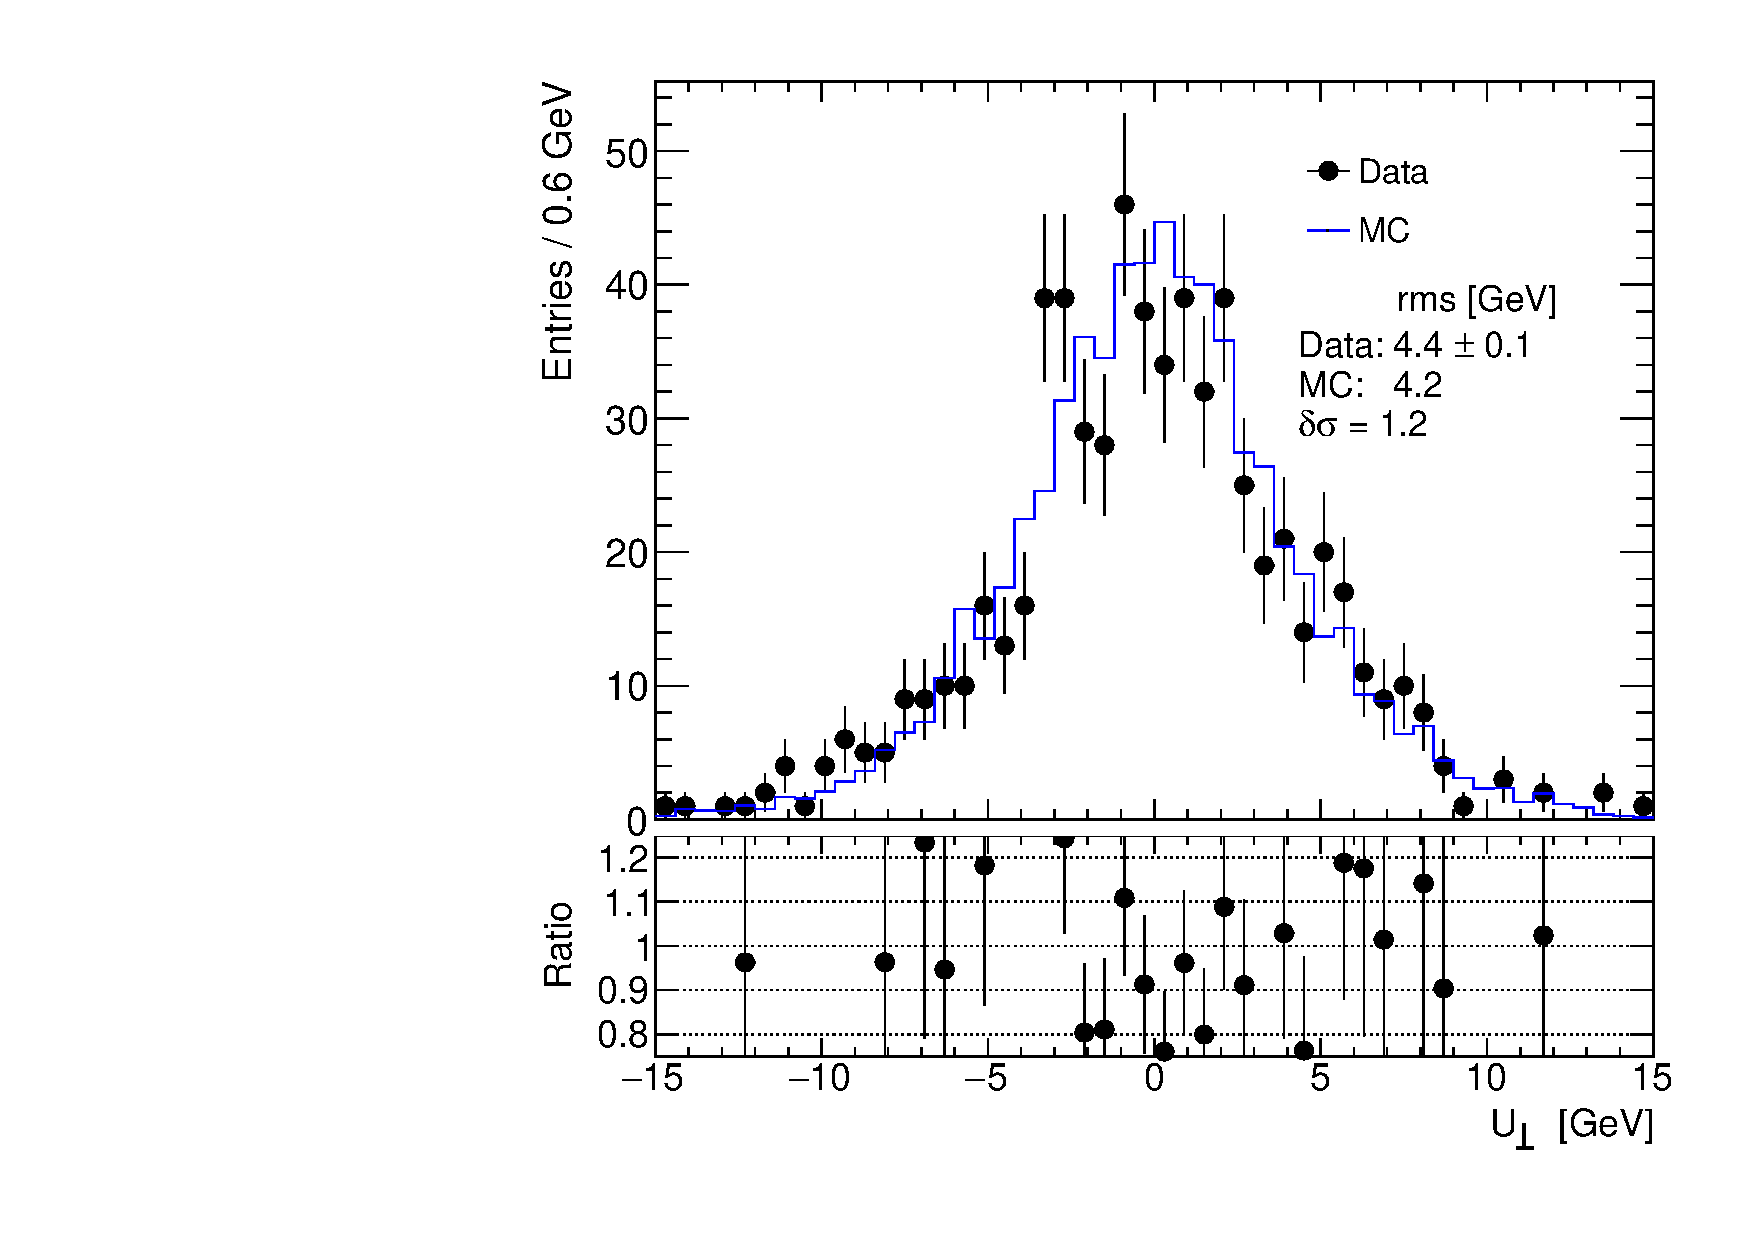
\includegraphics[width=1.\linewidth]{HadronRecoil/UPerpMRMS.pdf} \\ b)}
\end{minipage}
\vfill
\begin{minipage}[h]{0.40\linewidth}
\center{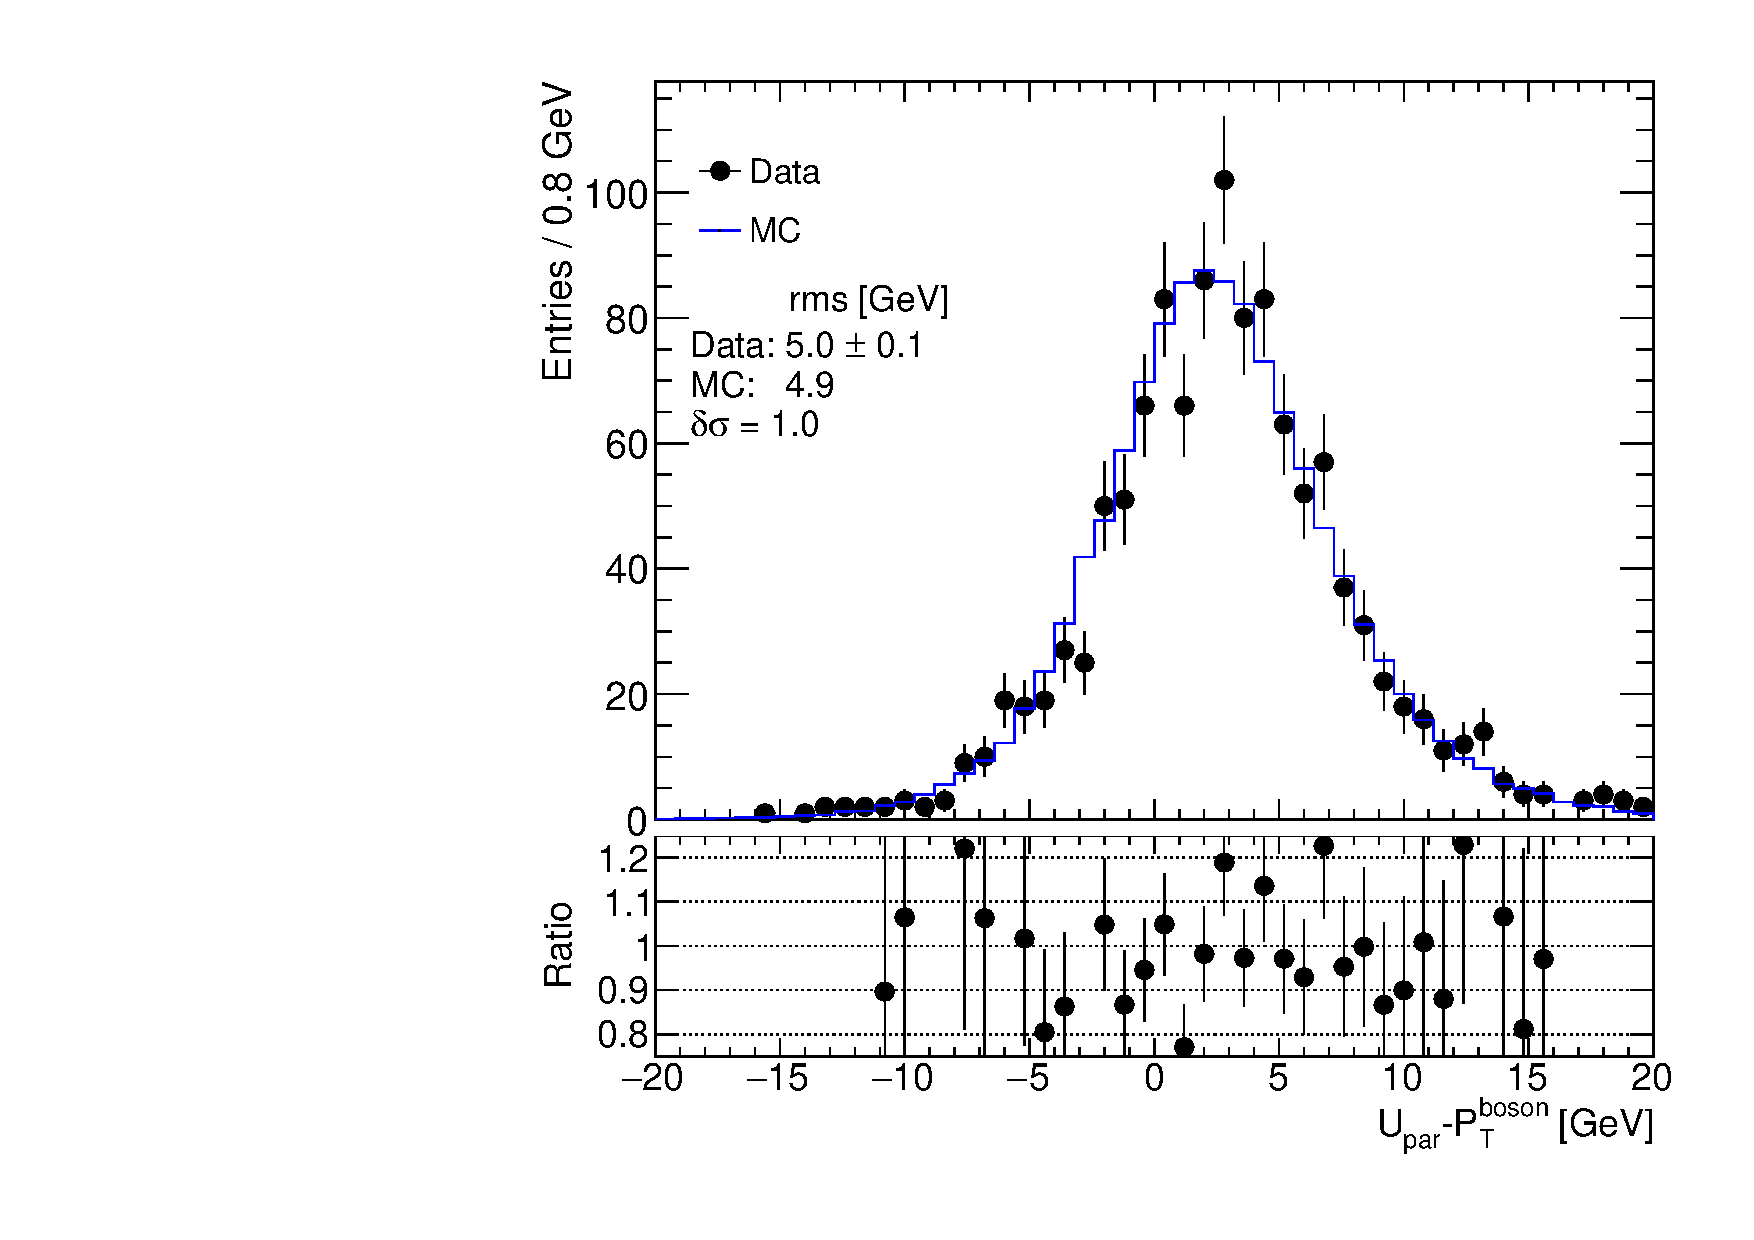
\includegraphics[width=1.\linewidth]{HadronRecoil/UParTotalRMS.pdf} \\ a)}
\end{minipage}
\hfill
\begin{minipage}[h]{0.40\linewidth}
\center{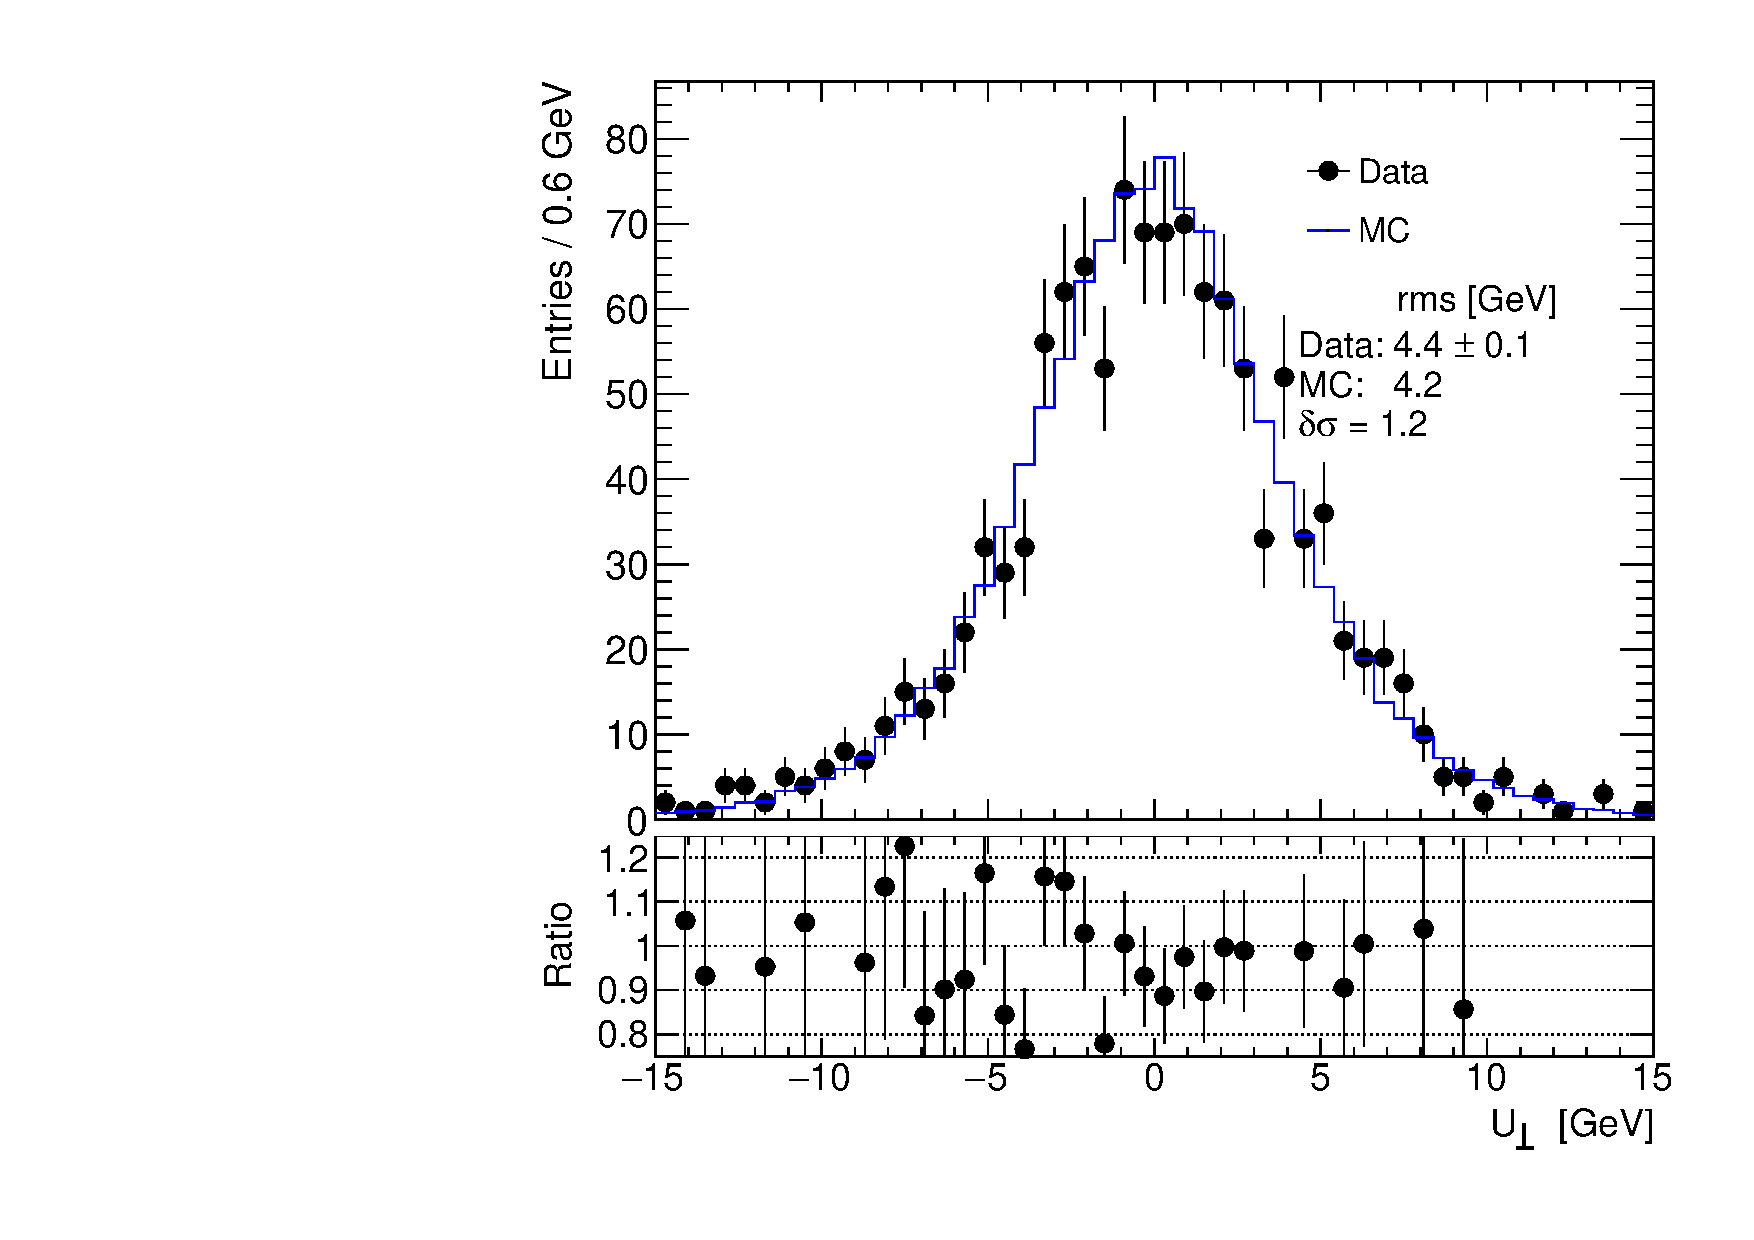
\includegraphics[width=1.\linewidth]{HadronRecoil/UPerpTotalRMS.pdf} \\ b)}
\end{minipage}
\caption{}
\label{HadrRecoil:CorrSumet}
\end{figure}

\begin{equation}
\upar' = \upar+Gaus(0, d\sigma)
\uperp' = \uperp + Gaus(0, d\sigma),
\end{equation}
where dSigma is a difference in a resoultions calculated as:
\begin{equation}
d\sigma=\sqrt{\sigma_{data}^2-\sigma_{MC}^2}
\end{equation}
Systematic error of this $d\sigma$ is taken as an statistical error for $\sigma_{data}$. Overall effect on a \cw depending on a $d\sigma$ is shown on a Fig. \ref{ris:CwSmear}.
Due to a random nature of this correction, effect is not stable for a small $d\sigma$. Stability of this correction can be tested by repeating this procedure several times with different random seed number. Overall effect on a \cw and corresponding systematical and statistical error are summarized in Tab. \ref{something}. The effect of stability of the correction is a subleading. 
\begin{figure}[h]
\begin{minipage}[h]{0.49\linewidth}
\center{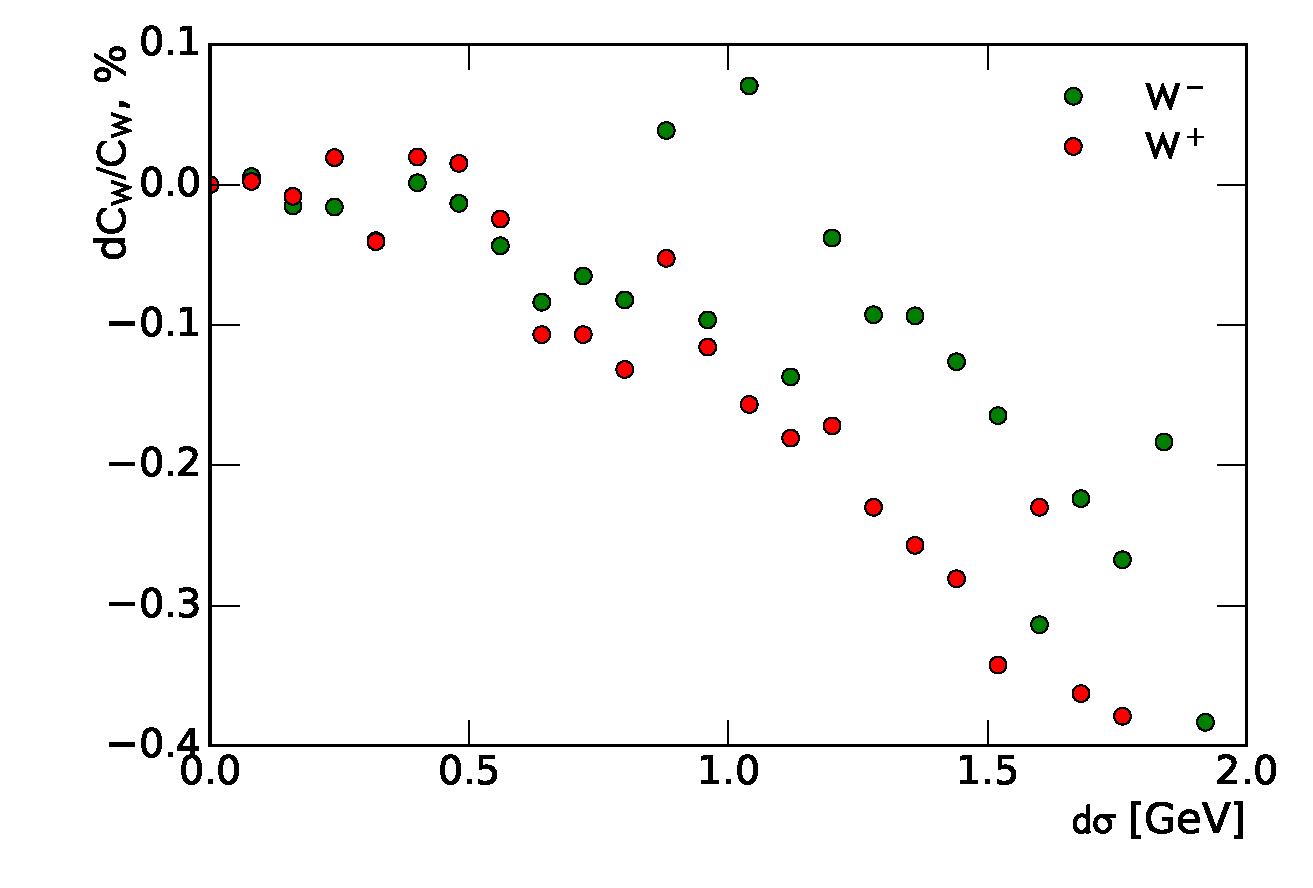
\includegraphics[width=1.\linewidth]{HadronRecoil/CWElectronSmearing.pdf} \\ a)}
\end{minipage}
\hfill
\begin{minipage}[h]{0.49\linewidth}
\center{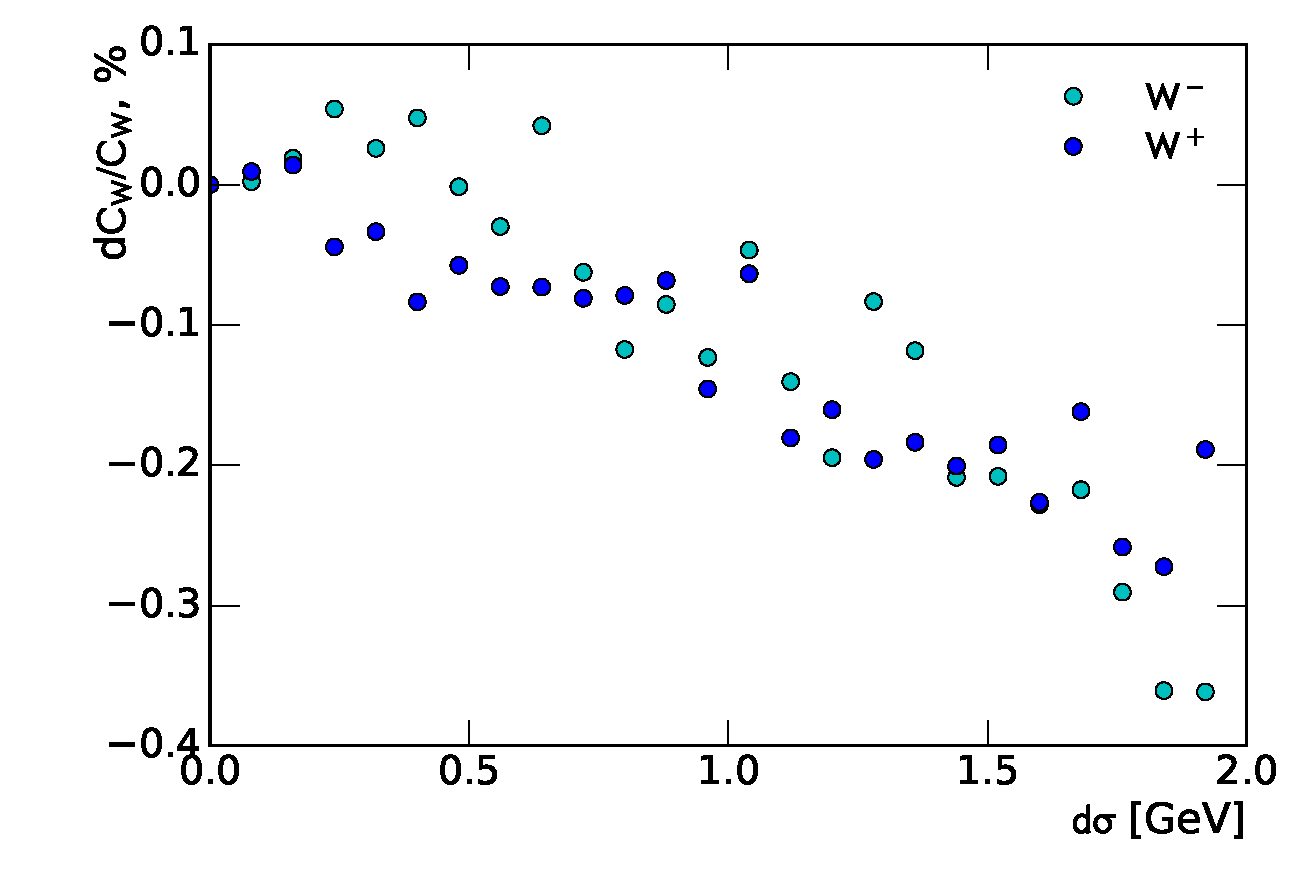
\includegraphics[width=1.\linewidth]{HadronRecoil/CWMuonSmearing.pdf} \\ b)}
\end{minipage}
\caption{Effect on a \cw for a different $d\sigma$ for a) \wenu b)\wmunu channel}
\label{ris:CwSmear}
\end{figure}

\subsection{Hadron recoil bias correction}

\begin{figure}[!htb]
\minipage{0.32\textwidth}
  \center{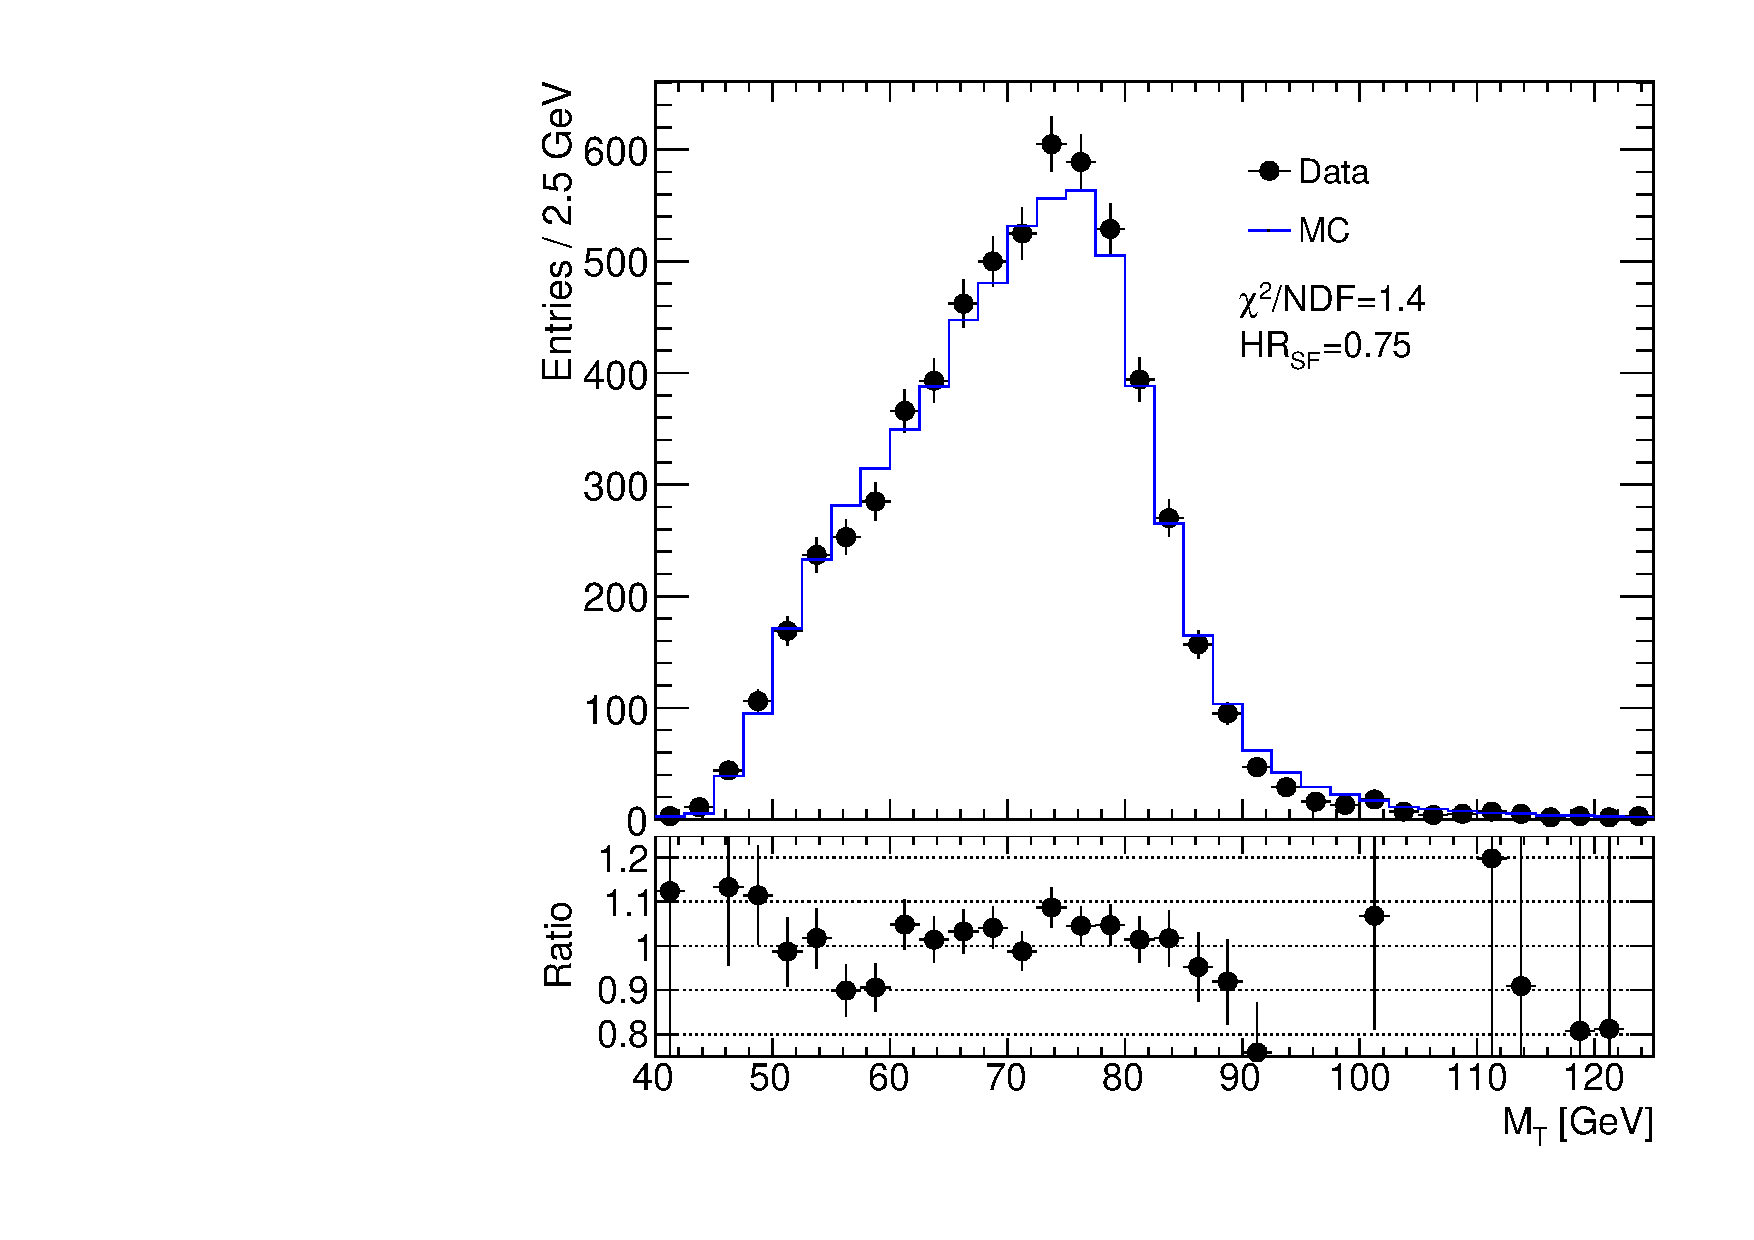
\includegraphics[width=\linewidth]{HadronRecoil/MtWEScale0.pdf} a)}
\endminipage\hfill
\minipage{0.32\textwidth}
   \center{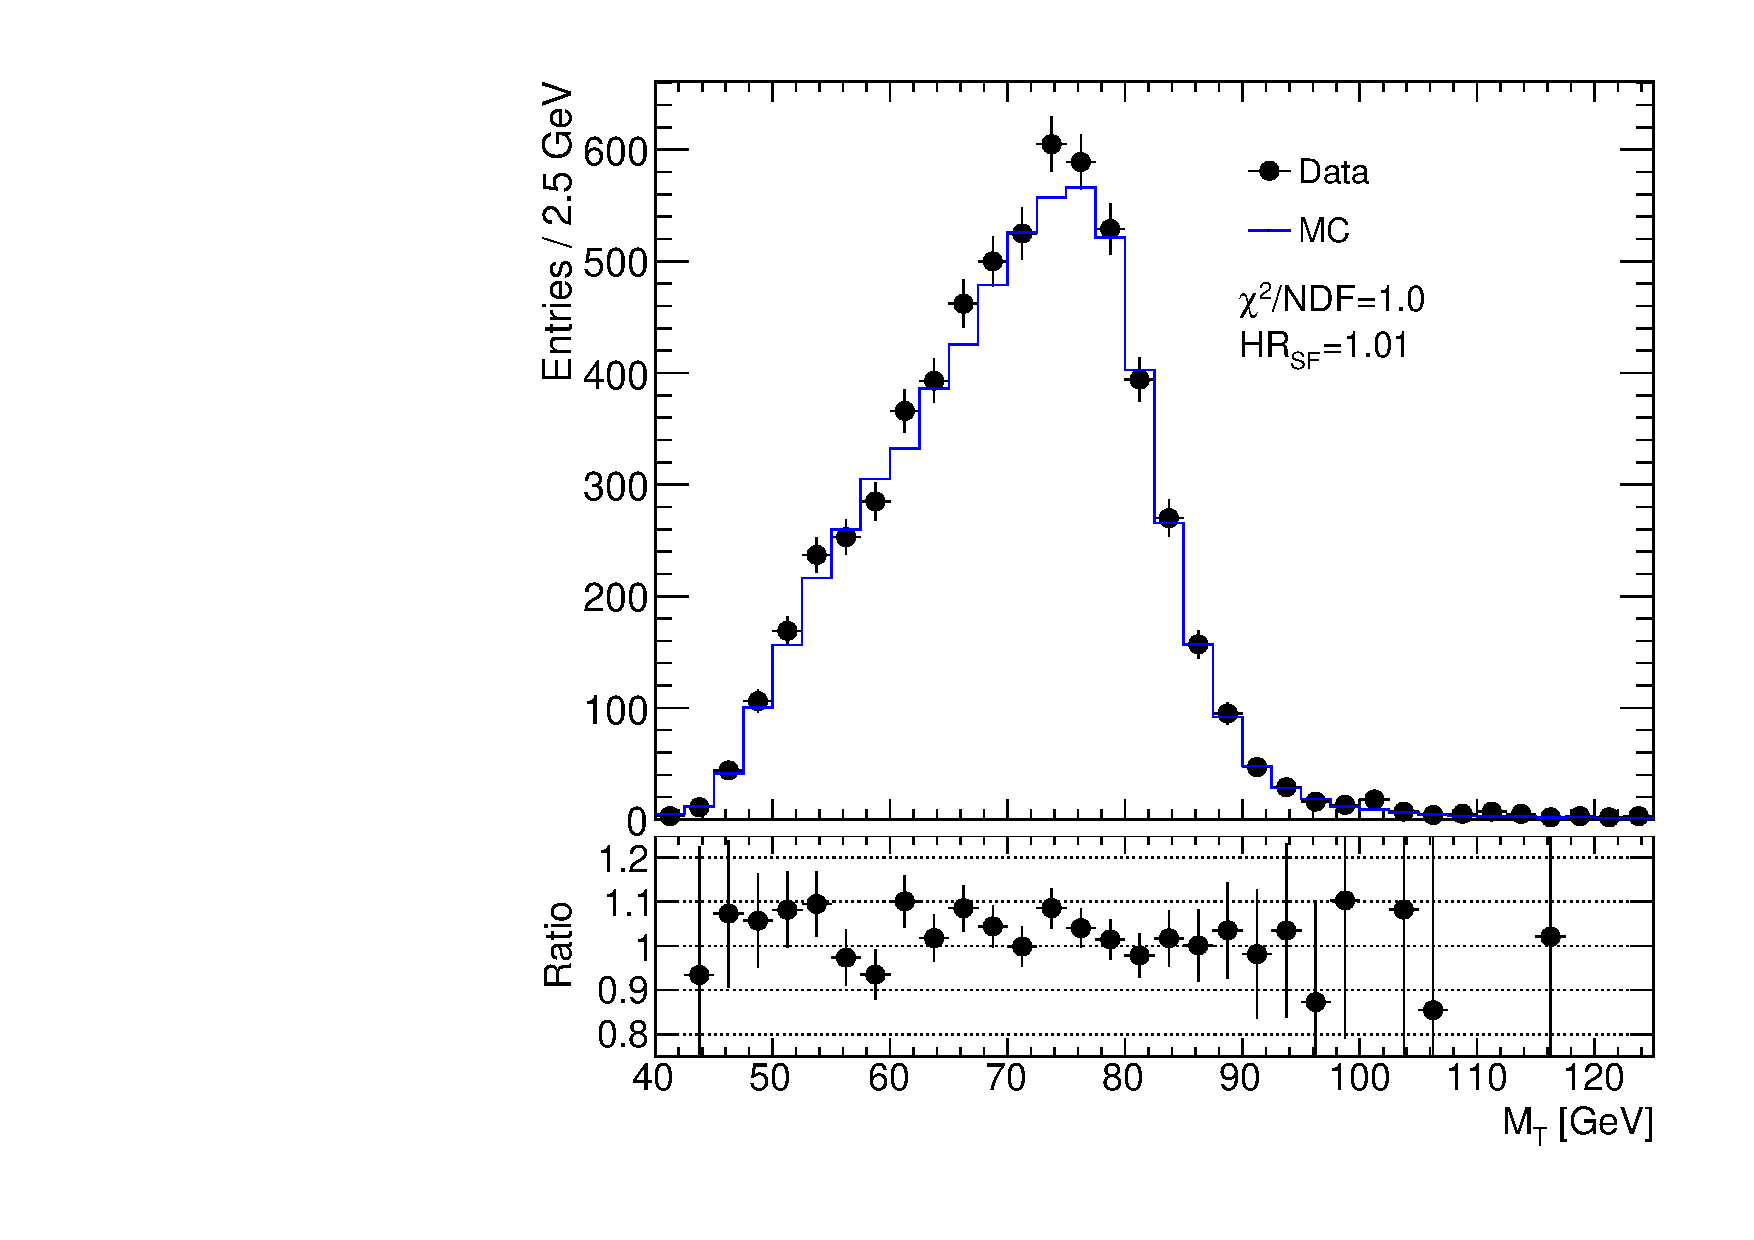
\includegraphics[width=\linewidth]{HadronRecoil/MtWEScale13.pdf} b)}
\endminipage\hfill
\minipage{0.32\textwidth}%
   \center{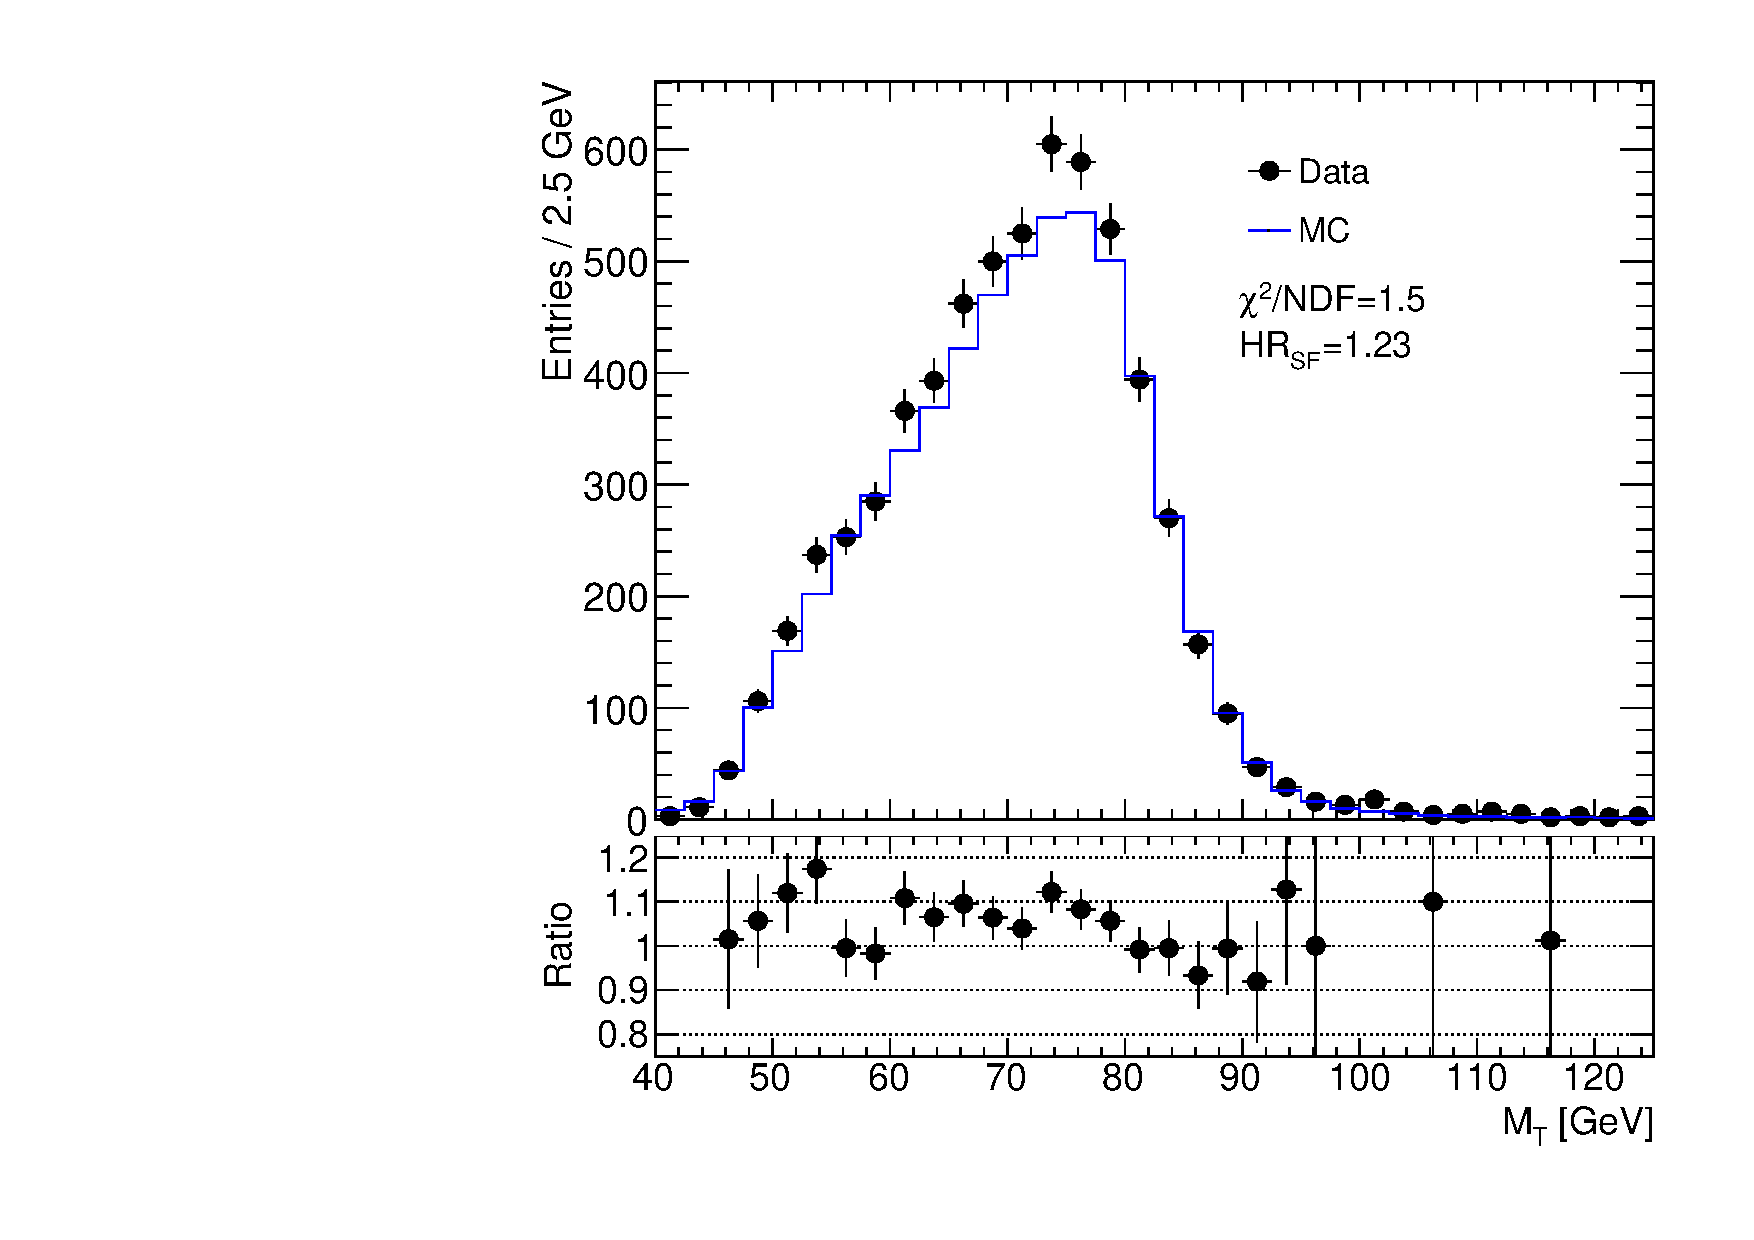
\includegraphics[width=\linewidth]{HadronRecoil/MtWEScale24.pdf} c)}
\endminipage
\vfill
\minipage{0.32\textwidth}
  \center{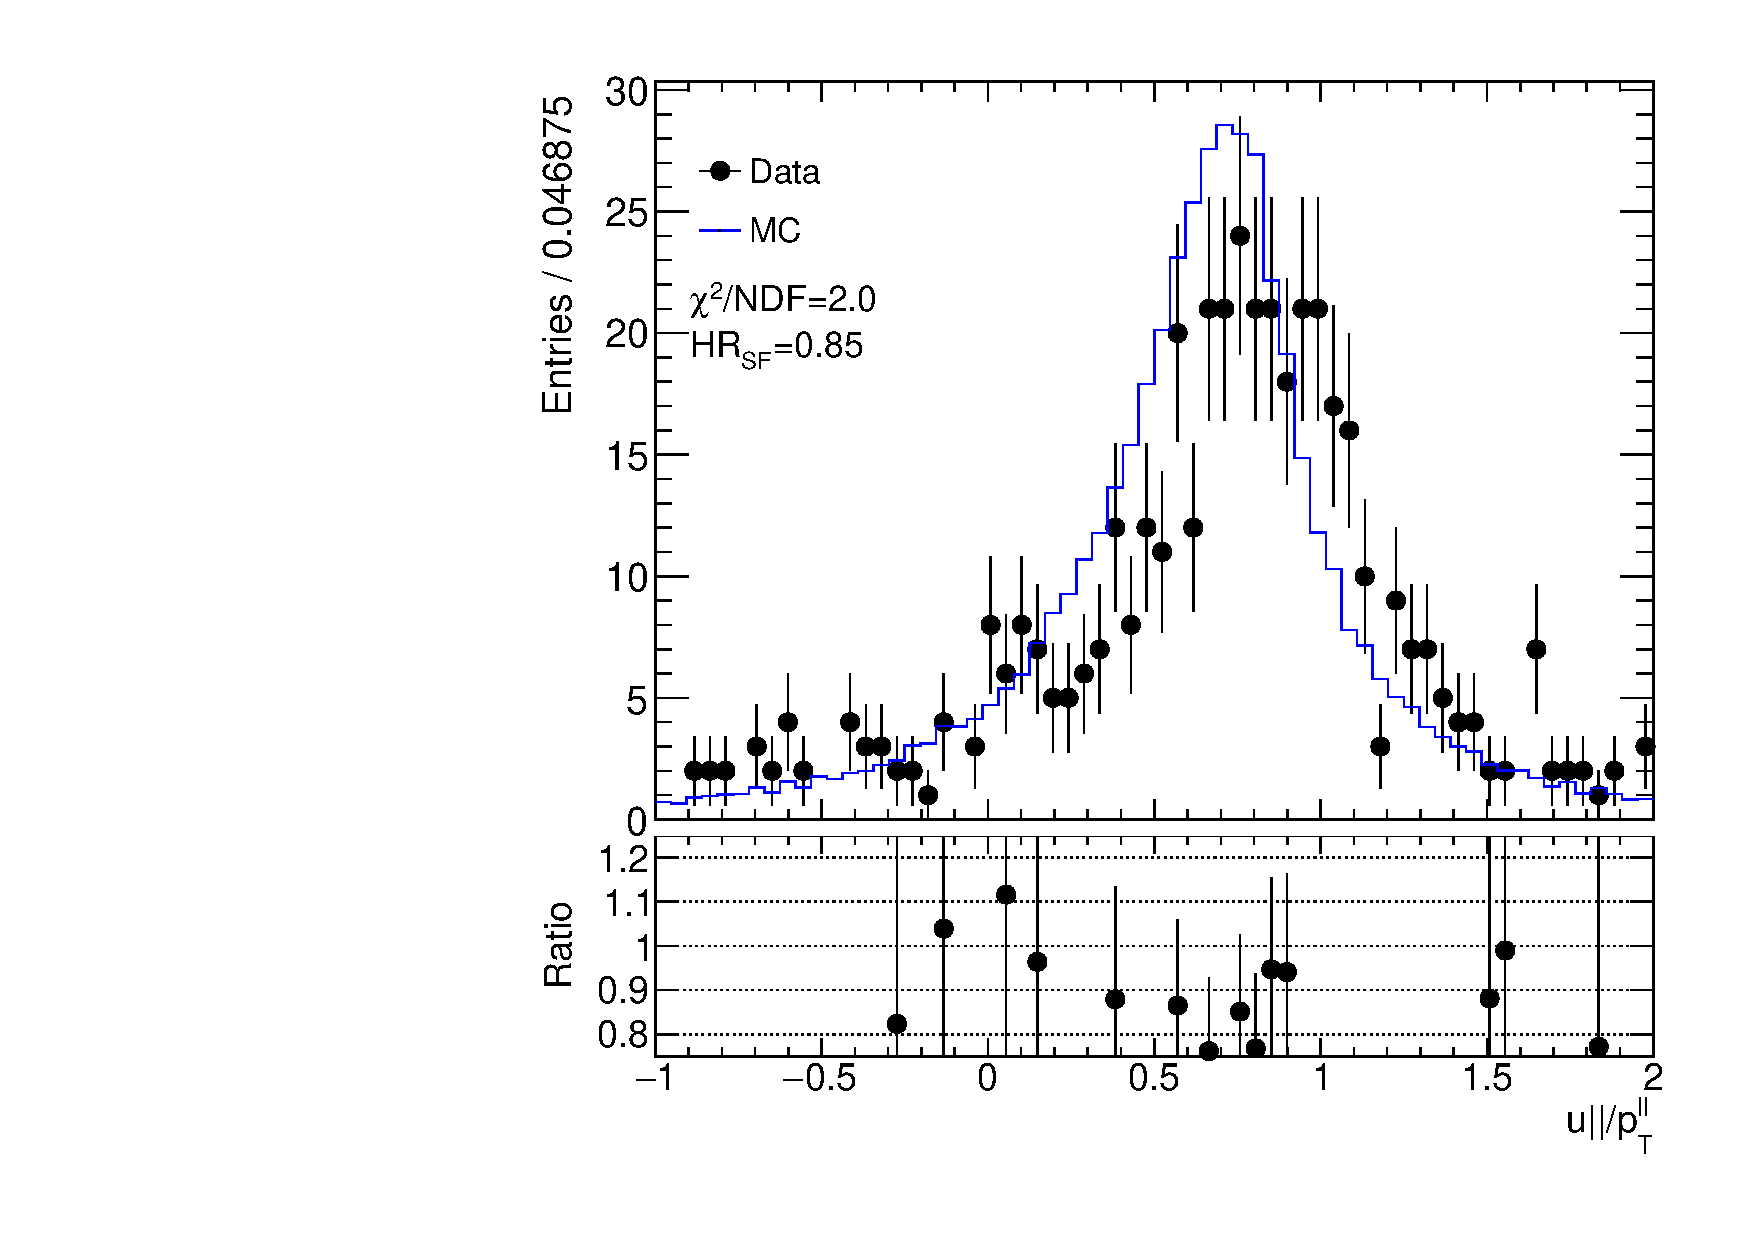
\includegraphics[width=\linewidth]{HadronRecoil/UParEScale5.pdf} a)}
\endminipage\hfill
\minipage{0.32\textwidth}
   \center{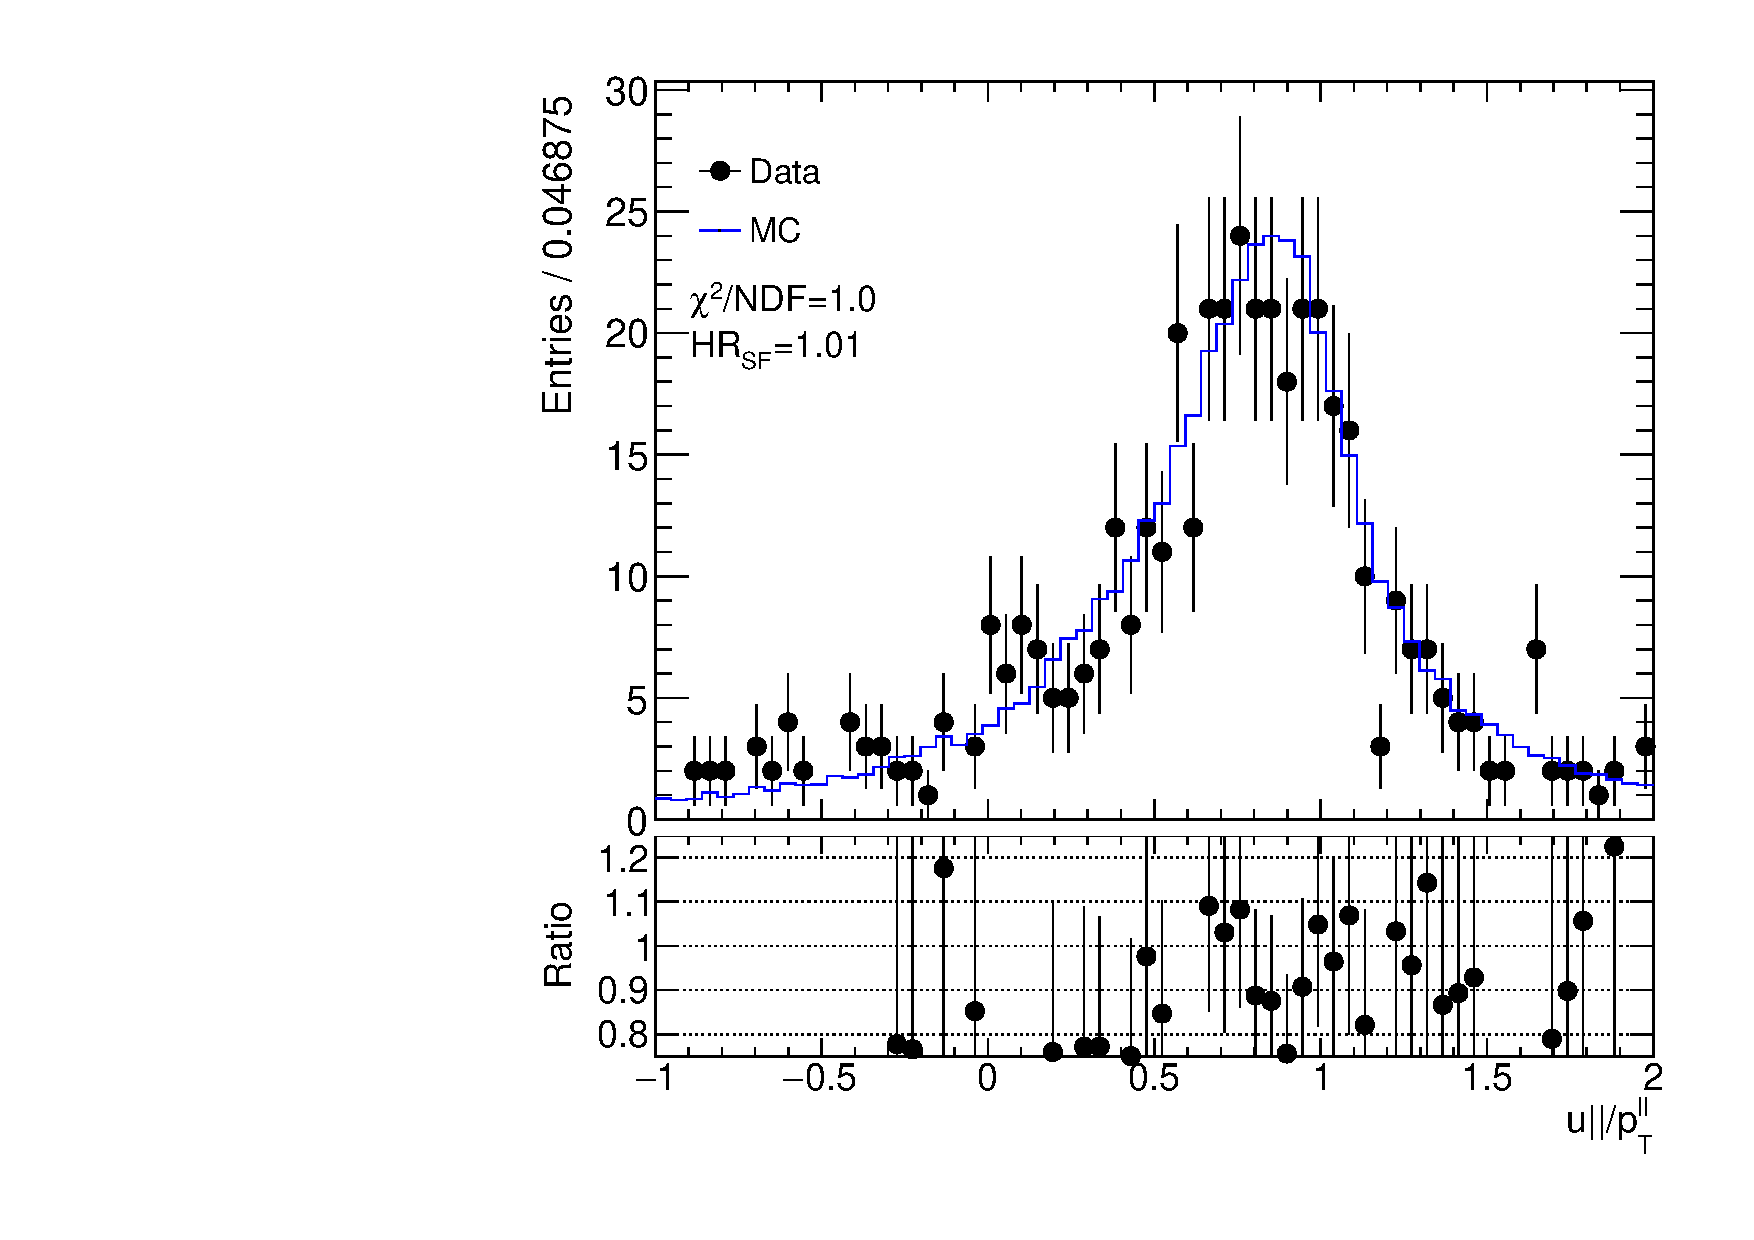
\includegraphics[width=\linewidth]{HadronRecoil/UParEScale13.pdf} b)}
\endminipage\hfill
\minipage{0.32\textwidth}%
   \center{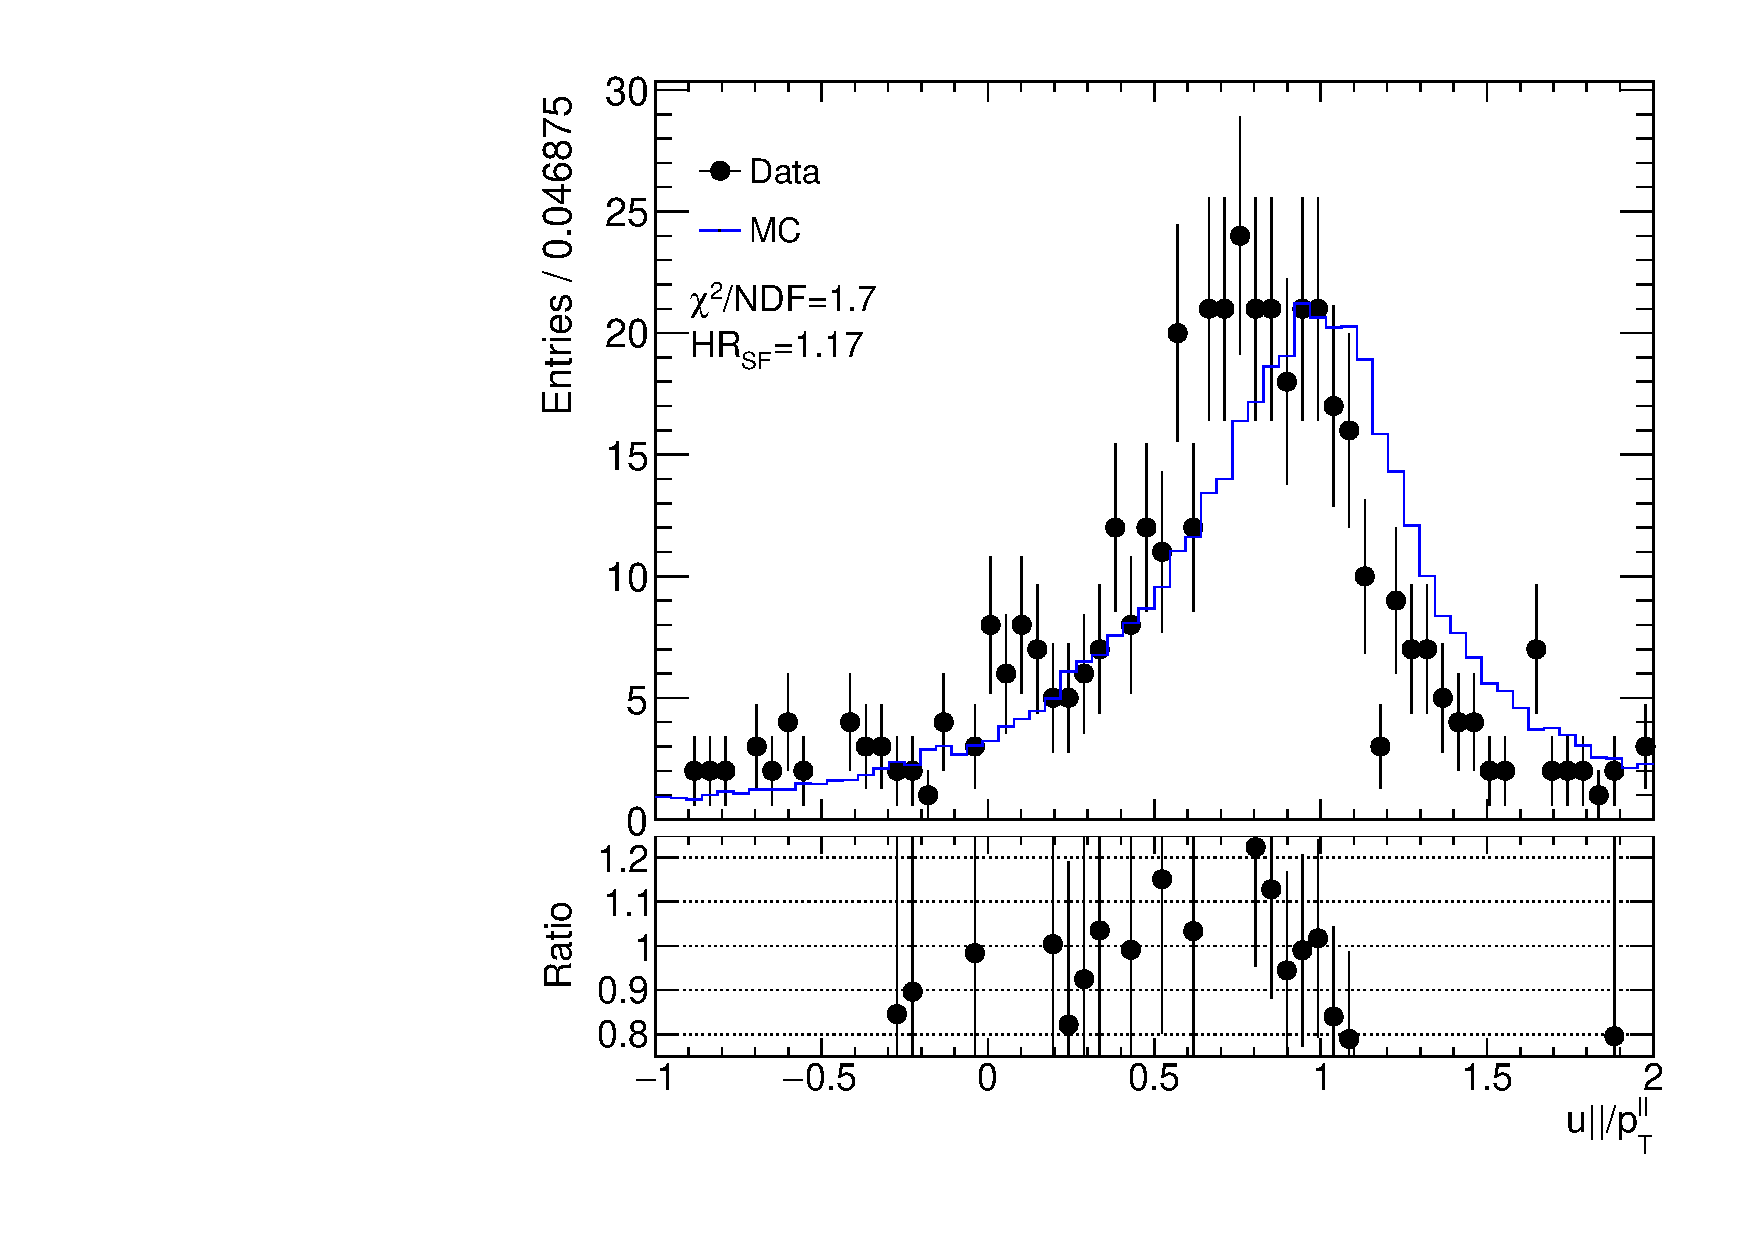
\includegraphics[width=\linewidth]{HadronRecoil/UParEScale21.pdf} c)}
\endminipage
\caption{Trigger scale factors for a) $\mu$ b) $\mu^{+}$  c) $\mu^{-}$}
\label{fig:MuSF}
\end{figure}
As it was mentioned before, it is possible to use both Z and W boson sample for hadron recoil bias determination. Correction factor $SF_{HR,bias}$ is applied as:
\begin{equation}
\upar^{MC,cor}=\upar^{MC} \cdot SF_{HR,bias},
\end{equation}

\begin{figure}[h]
\begin{minipage}[h]{0.49\linewidth}
\center{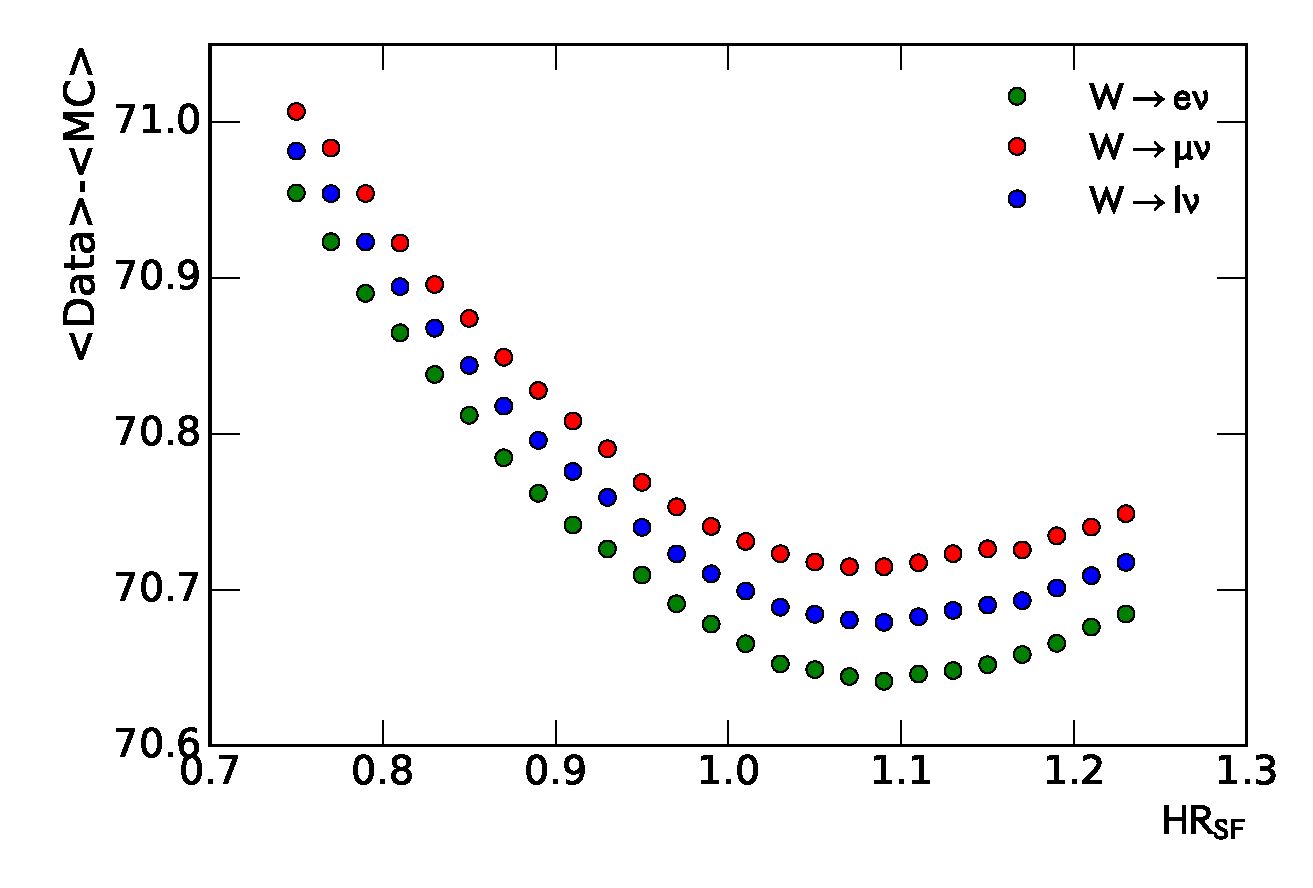
\includegraphics[width=1.\linewidth]{HadronRecoil/MeanAll.pdf} \\ a)}
\end{minipage}
\hfill
\begin{minipage}[h]{0.49\linewidth}
\center{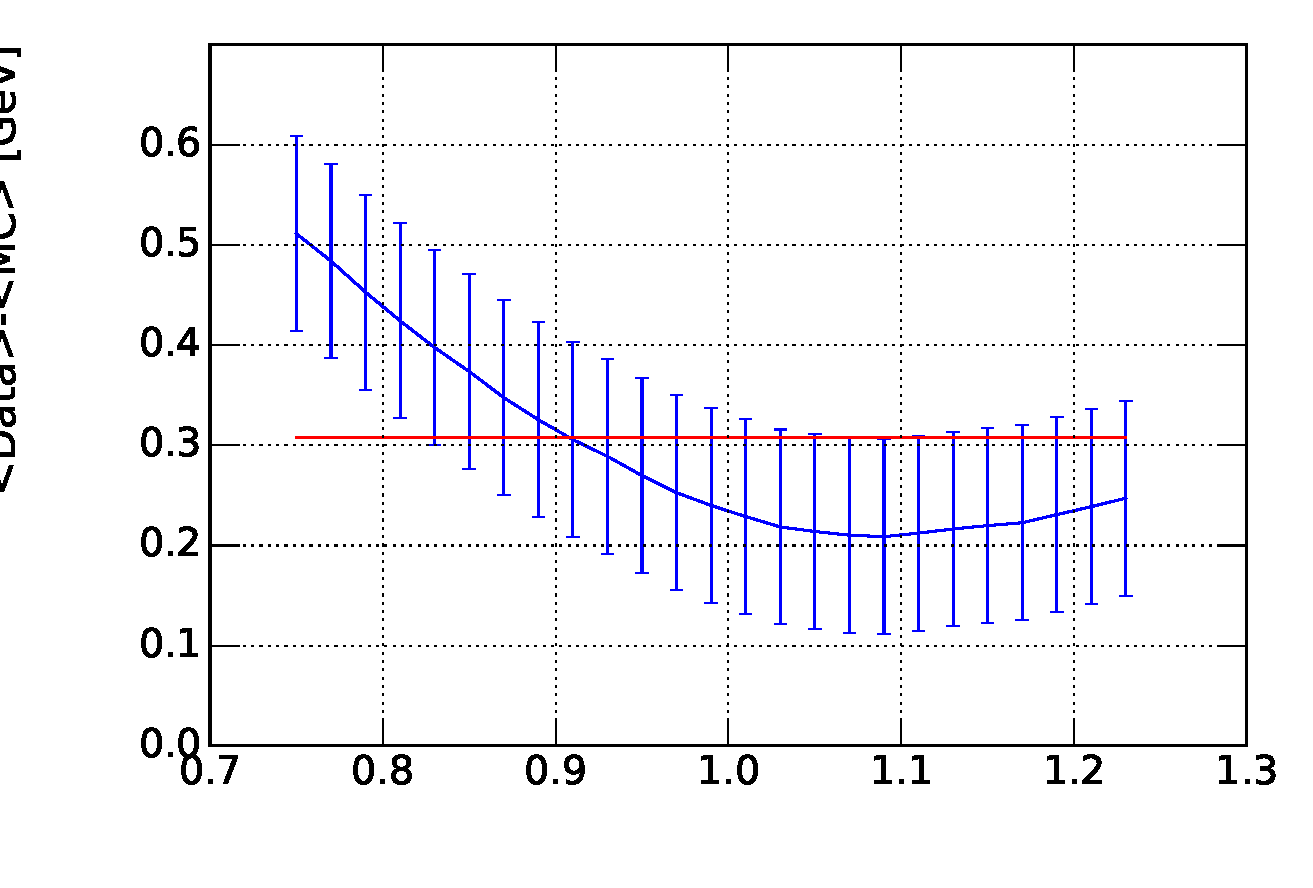
\includegraphics[width=1.\linewidth]{HadronRecoil/MeanCombined.pdf} \\ b)}
\end{minipage}
\vfill
\begin{minipage}[h]{0.49\linewidth}
\center{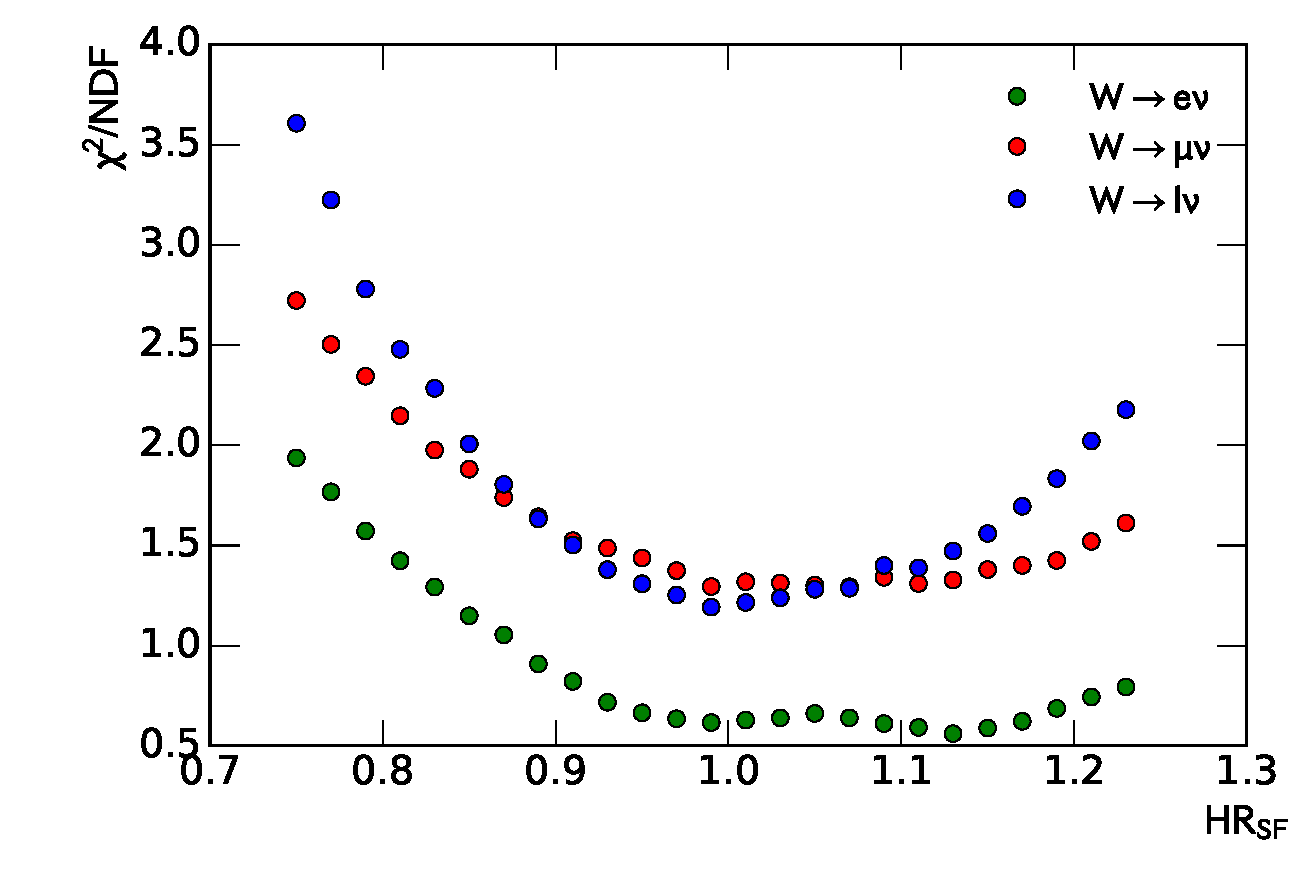
\includegraphics[width=1.\linewidth]{HadronRecoil/chi2AllChannelsMtw.pdf} \\ a)}
\end{minipage}
\hfill
\begin{minipage}[h]{0.49\linewidth}
\center{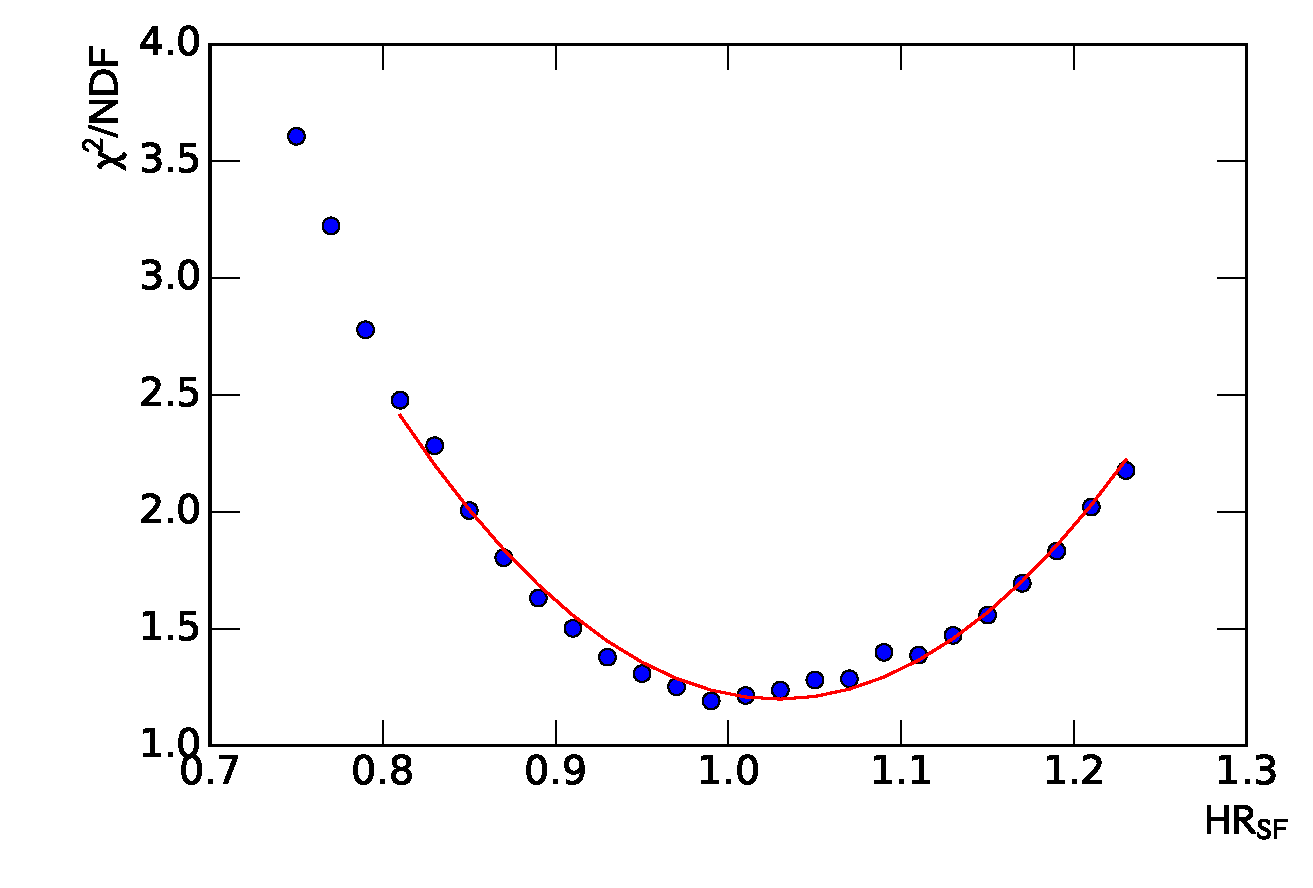
\includegraphics[width=1.\linewidth]{HadronRecoil/chi2TotalMtw.pdf} \\ b)}
\end{minipage}
\vfill
\begin{minipage}[h]{0.49\linewidth}
\center{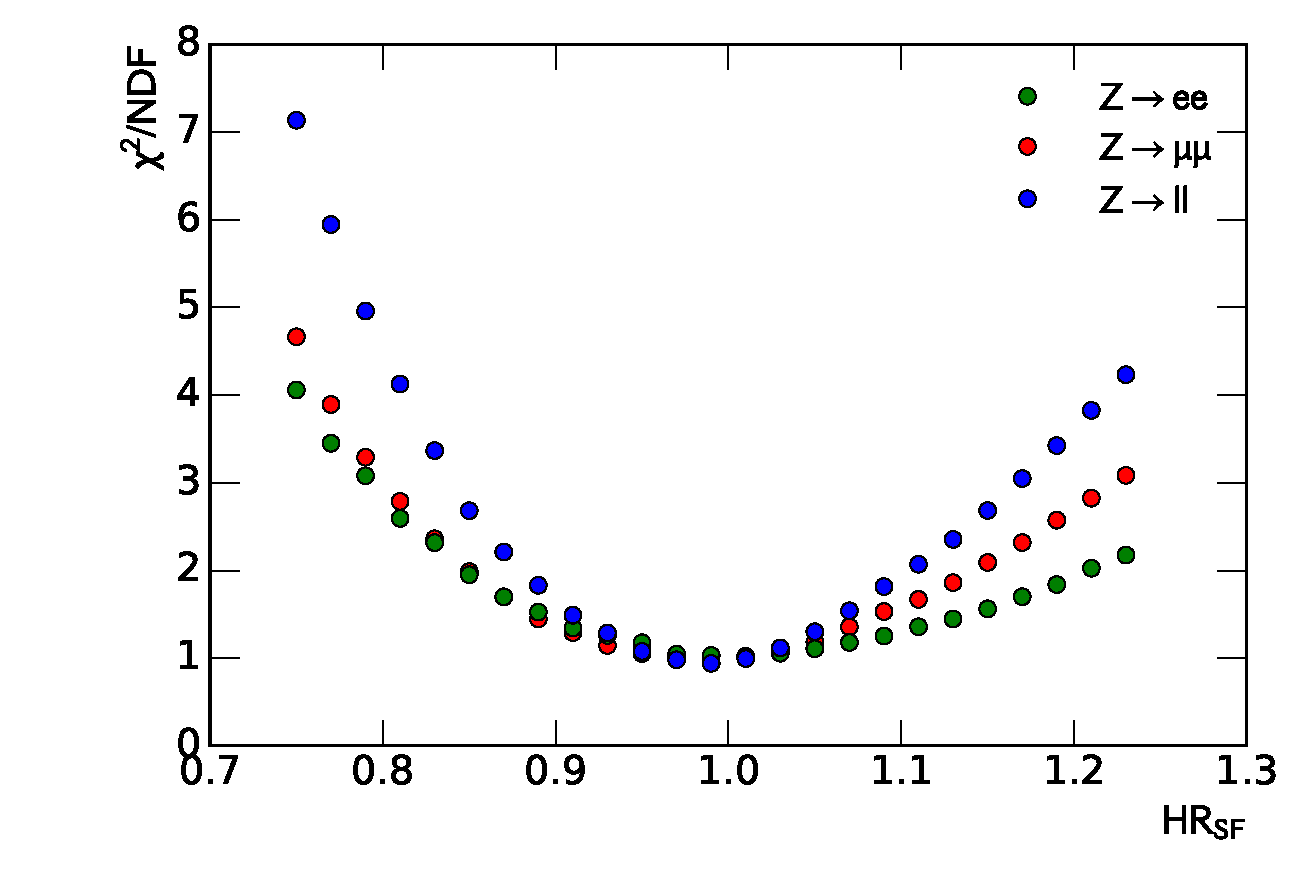
\includegraphics[width=1.\linewidth]{HadronRecoil/chi2Upar.pdf} \\ a)}
\end{minipage}
\hfill
\begin{minipage}[h]{0.49\linewidth}
\center{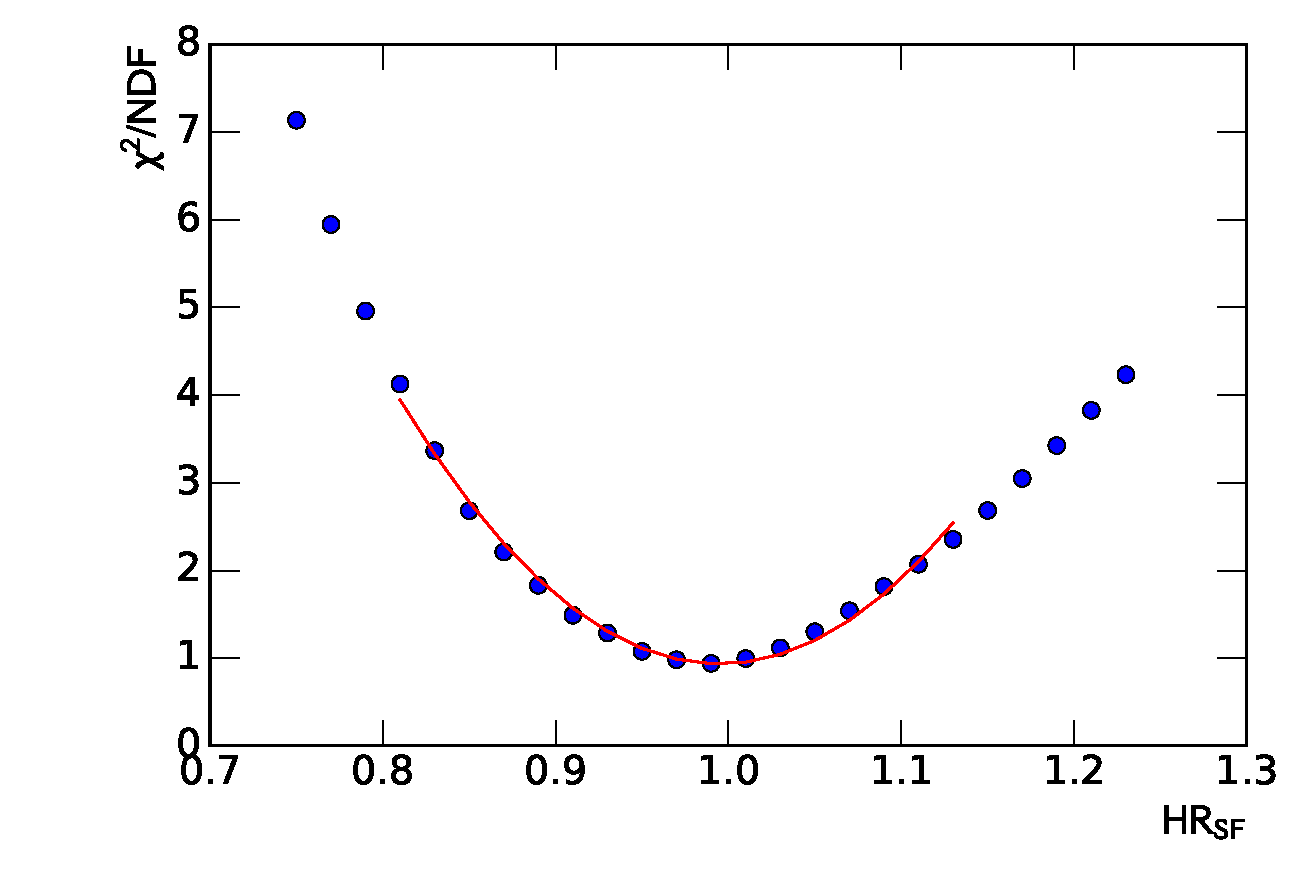
\includegraphics[width=1.\linewidth]{HadronRecoil/chi2UparTot.pdf} \\ b)}
\end{minipage}
\caption{Effect on a \cw for a different $d\sigma$ for a) \wenu b)\wmunu channel}
\label{ris:Cw}
\end{figure}
and can be obtained by scanning the impact of the scaling factor on the Data to MC agreement of the distributions that are dominated by the recoil scale uncertainties. Since W boson has no second source of \ptw measurments, determination of the hadron recoil bias should use the distributions, that  are not sensitive to a truth \ptw spectrum.  One of the optimal choises is a \mtw distribution. Transverse mass distribution for a different scale choises is shown on a Fig. \ref{HadronRecoilScaleMtW}. Multijet background is not included, because it shape and number of events is depending on a hadron recoil scale and thus can introduce additional systematics.

The first way to determine correction factor is using a difference in the mean of transverse mass in data and MC. Statistical error of this determination is an error of the mean in the data. The precision of this method is low, is it is mainly used as a cross-check. 

Second way is calculating \chiD for each correction factor. The ideal correction factor is determined by fitting \chiD distribution by the function:
\begin{equation}
\chi^2 = \frac{(x-sf_{best})^2}{\sigma_{sf}^2}+\chi^2_0,
\end{equation}
where $sf_{best}$ is the best scale factor and $\sigma_{sf}$ is a statistical error of this parameter. Distribution of \chiD and a fit in combined W channel is shown on a Fig. \ref{mtWChi2}.

Because of the possible mismodelling of the tail \mtw distribution it is not included in a \chiD calculation, leaving a free choise of the parameter of the cutoff.  It is also possible to exclude regions with high multijet background contamination by applying a tighter cut on a \mtw. 
This fit range is introducing one source of systematic error. Effect of the range on value determination is shown on a Fig. \ref{ScaleMtWRange}. 
Similarly to a W channel, scale correction in a Z sample can be determined from distribution $\frac{\upar}{p_T^{ll}}$, shown on a Fig. \ref{uPAr}. 
Since there is no choise of the range and dependency on $P_T^{bos}$ modelling, there is just one source of uncertainty.
  
Results on a hadron scale factros and it's errors are shown in a Table \ref{tab:SFHadronRecoil}. The results are consistent within 1 sigma. 

\begin{figure}[h]
\begin{minipage}[h]{0.49\linewidth}
\center{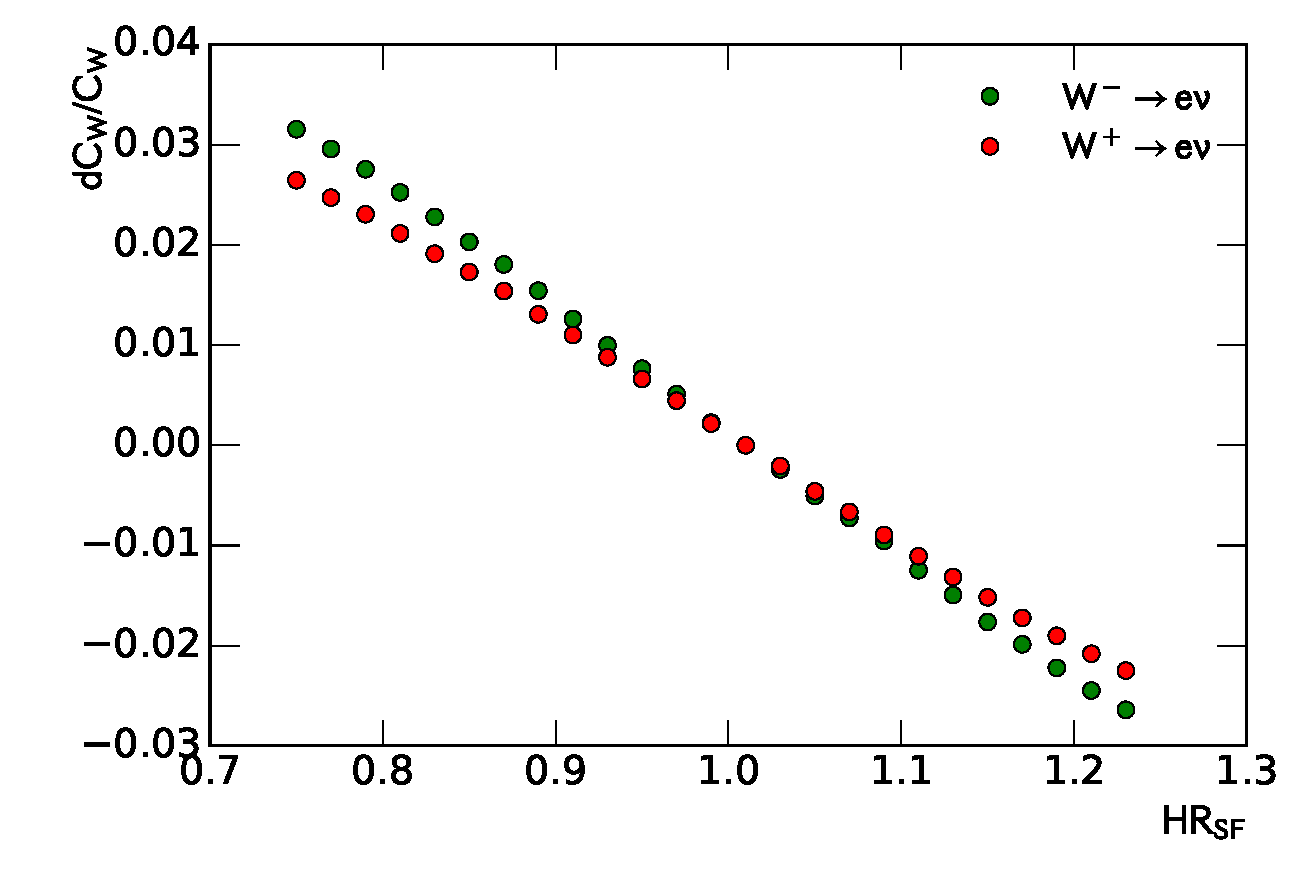
\includegraphics[width=1.\linewidth]{HadronRecoil/CWElectron.pdf} \\ a)}
\end{minipage}
\hfill
\begin{minipage}[h]{0.49\linewidth}
\center{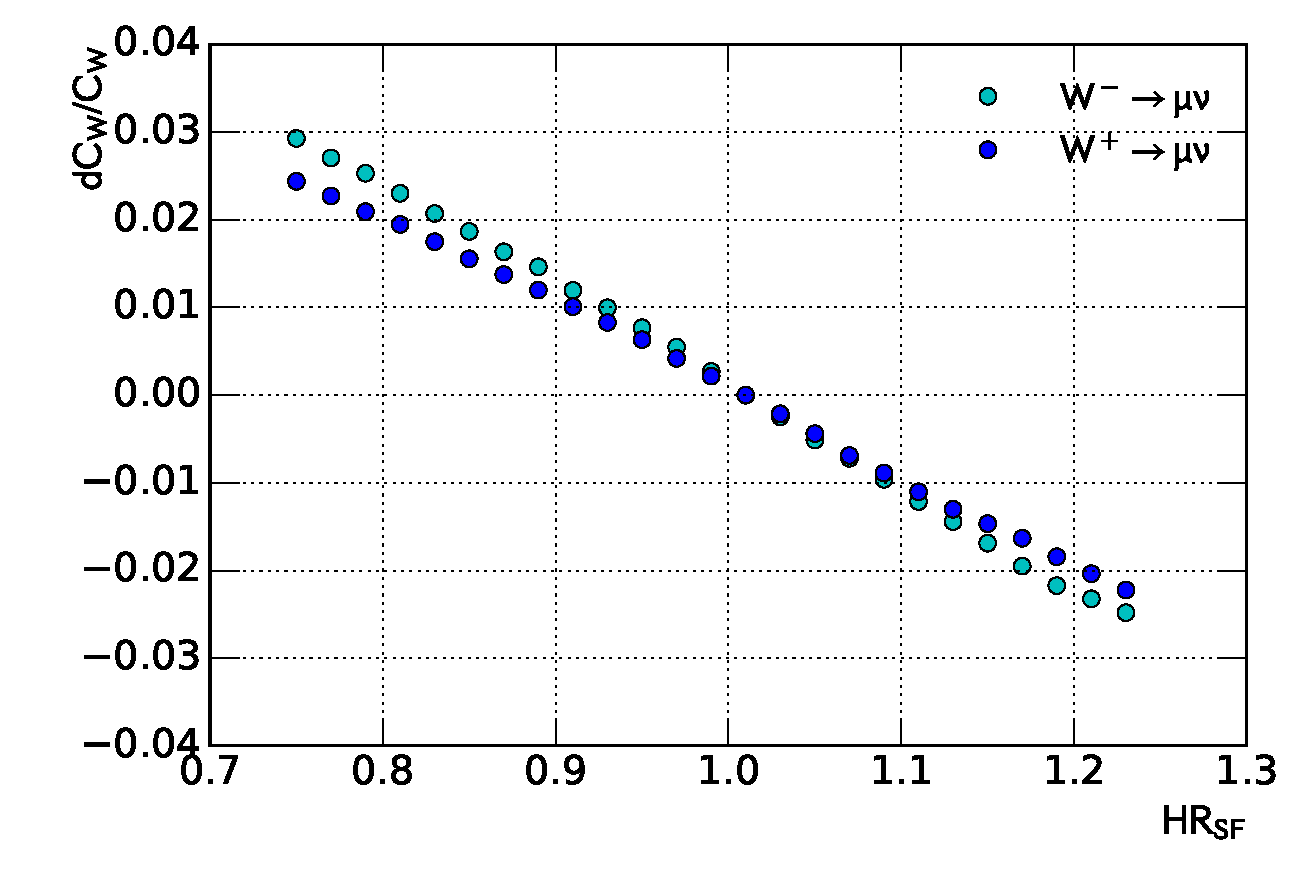
\includegraphics[width=1.\linewidth]{HadronRecoil/CWMuon.pdf} \\ b)}
\end{minipage}
\caption{Effect on a \cw for a different $d\sigma$ for a) \wenu b)\wmunu channel}
\label{ris:Cw}
\end{figure}

\begin{table}
\begin{center}
\begin{tabular}{| l | c | c |}
\hline
Method & SF & error \\
\hline
\hline
Mean $M_T^{W}$ & 1.10 & 0.2\\
$M_T^{W}$ \chiD & 1.01 & 0.07 \\
\upar \chiD & 1.00 & 0.014 \\
\hline
Total & 1.010 & 0.013 \\
\hline
\end{tabular}
\end{center}
\end{table}
